%----------------------------------------------------------------------------------------------------------
\chapter{Theoretical background}%
\label{chap:introduction_to_vsas}
%----------------------------------------------------------------------------------------------------------

In this chapter, we present the theoretical background and mathematical formalism needed as basis for later chapters.
We introduce \acfp{VSA}, describe their most important properties and present proofs where relevant for the thesis.
We proceed with one particular instantiation of \ac{VSA}, the \acf{SPA}, and present more specific properties, which do not necessary hold for all \acp{VSA}.
Additionally, we give a brief introduction to the theory of the \acf{NEF}, a set of mathematical tools enabling the implementation of the \ac{SPA} in \acp{SNN}.
Then, we shift our focus to cognitive modeling based on such vector representations keeping it as generic as possible without particular attention on the \ac{SPA}. 
We show several approaches to generate vector vocabularies, which form the basis of more complex structured representations built from them using the \ac{VSA}'s algebraic operations.
Bringing all of the presented tools together, we show how the \ac{NEF} can be used to implement vector representation generated using the \ac{SPA} in a spiking neuron substrate.

%----------------------------------------------------------------------------------------------------------
\section{Mathematical properties of \aclp{VSA}}
\label{sec:math_prop_vsas}
%----------------------------------------------------------------------------------------------------------

The term \acp{VSA} - first coined by Ross W. Gayler \cite{Gayler2003} - refers to a class of similar approaches for cognitive modeling making use of distributed representations.
The basic idea behind all of those approaches is to represent structure (e.g.\ cognitive concepts, symbols or language) in a high-dimensional vector space by mapping each entity to be represented to a (possibly random) vector.
One of the most important properties of high-dimensional vector spaces enabling this kind of representation is the fact, that two high-dimensional random vectors are likely to be dissimilar.
In the following, we will show what we mean by fuzzy terms like \emph{dissimilar} or \emph{likely} and provide more precise statements.

One main requirement in the context of cognitive modeling is the ability of the modeling framework to address the binding problem \cite{Treisman1999}.
In \cite{Jackendoff2002}, Jackendoff phrases this as the problem of "combining independent bits into a single coherent percept".
One strength of \acp{VSA} is that they offer the possibility to manipulate their entities (i.e., vectors) through algebraic operations, usually at least one \emph{addition-like} and \emph{multiplication-like} operation each.
Typically, the multiplication operation is used for binding different representations into a new vector.
This operation, depending on the vector representation, is constructed with some desirable properties in mind (see Definition~\ref{def:binding}).
A first attempt on using a multiplication operation on vectors for binding was done by Smolensky \cite{Smolensky1990} using the tensor product.
The major drawback of this approach is exploding dimensionality of the tensor product.
For finite dimensional vector spaces  $V$ and $W$ of dimensions $n$ and $m$, the tensor space $V \otimes W$ is a vector space of dimension $n\cdot m$.
As a consequence, each binding operation $v\otimes w$ for vectors $ \mathbf{v} \in V, \mathbf{w} \in W$ would increase the dimension of the representational space, which is computationally unfeasible and leads to poor scaling.
This lead researchers to define several slightly different multiplication or binding operations, depending on the underlying numerical structure.
The most prominent examples are element-wise multiplication in Gayler's \ac{MAP}-architecture \cite{Gayler1998}, the XOR-operation in Kanerva's \acp{BSC} \cite{Kanerva2000, Kanerva2009} as well as circular convolution in Plate's \acp{HRR} \cite{Plate1991, Plate1994}.

\begin{defn}
	\label{def:VSA}
	Let $N \subseteq K$ be a subset of some number field $K$ (i.e.\ a set of numbers) and $D \in \mathbb{N}$ a natural number.
	Furthermore, let
	\[V_{D}(N)=\{ \mathbf{x}=\left(x_{0}, \cdots, x_{D-1}\right)  | x_{i} \in N\} \subseteq K^{D}\]
	be the set of all $D$-tuples with entries in $N$.
	Let
	\begin{align*}
		&\abb{\oplus}{V_{D}(N) \times V_{D}(N)}{K^{D}}{( \mathbf{v}, \mathbf{w})}{\oplus( \mathbf{v}, \mathbf{w}) =: \mathbf{v}\oplus \mathbf{w}}, \\
		&\abb{\varoast}{V_{D}(N) \times V_{D}(N)}{K^{D}}{( \mathbf{v}, \mathbf{w})}{\varoast( \mathbf{v}, \mathbf{w}) =: \mathbf{v}\varoast \mathbf{w}}
	\end{align*}
	be functions with $\oplus$ following the rules of ordinary addition - namely commutativity, associativity, existence of a neutral element and existence of inverse elements - and for any elements $ \mathbf{u}, \mathbf{v}, \mathbf{w} \in V_{D}(N)$
	\[ \mathbf{u} \varoast ( \mathbf{v} \oplus \mathbf{w}) = \mathbf{u} \varoast \mathbf{v} \oplus \mathbf{u} \varoast \mathbf{w}.\]
	If there is furthermore a distinct element $\pmb{1} \in V_{D}(N)$ with
	\[ \mathbf{v} \varoast \pmb{1} = \pmb{1} \varoast \mathbf{v} = \mathbf{v}\]
	for any $v \in V_{D}(N)$ and a function $\abbil{\phi}{V_{D}(N) \times V_{D}(N)}{\left[-1,1\right]}$, we call $(V_{D}(N), \varoast, \oplus, \phi)$ a \emph{\acrfull{VSA}} of dimension $D$.
	The function $\phi$ is called a \emph{measure of similarity}.
	If $N$ is a subset of the real or complex numbers, i.e., $N \subset \mathbb{R}$ or $N \subseteq \mathbb{C}$, we call any \ac{VSA} $\left(V_{D}(N), \varoast, \oplus, \phi\right)$ \emph{continuous}.
\end{defn}
Although the set $V_{D}(N)$ might not be a vector space in the strict mathematical sense (in most cases it is at least a subset of a vector space), we will refer to its elements as \emph{vectors}.
%The metric in definition~\ref{def:VSA} is needed as measure of similarity between vectors.
Before we proceed in deriving some important properties of \acp{VSA}, we present some of the most prominent examples.

\begin{ex} \aclp{VSA}
	\label{ex:VSAs}
	\begin{enumerate}
		\item The first example of a \ac{VSA} is Kanerva's \acfl{BSC} \cite{Kanerva2009}.
            He restricts the elements of his vectors to binary values, i.e., $N=\{0,1\} = \mathbb{F}_{2}$.
		The operations $\varoast$ and $\oplus$ in this case are the XOR-function and a thresholded sum respectively.
		With $ \mathbf{v}_{i} = \left(v_{i 0}, \cdots, v_{i D-1}\right) \in V_{D}(N)$ and  $i \in \{1, \cdots, n\}$, the operation $\oplus$ is usually defined in the following way
		\begin{align*}
			\mathbf{v}_{1} \oplus \cdots \oplus \mathbf{v}_{n} =: &\mathbf{x} = \left(x_{0}, \cdots, x_{D-1}\right) \textrm{ with } \\
			&x_{j}:= \begin{cases}
				1 & \sum\limits_{i=1}^{n} v_{ij} \geq \frac{n}{2} \\
				0 & \sum\limits_{i=1}^{n} v_{ij} < \frac{n}{2}
			\end{cases}.
		\end{align*}
		This definition ensures, that the results of the addition operation $\oplus$ remain binary.
		Usually, a normalized Hamming distance
		\[
		\phi( \mathbf{v}, \mathbf{w}) := 1 - \frac{2}{D} \left| \{ v_{i} \neq w_{i} | i \in \{0, \cdots, D-1\} \} \right|
		\]
		is used as a measure of similarity in this architecture.
		\acp{BSC} have some interesting properties compared to other \acp{VSA}:
		The neutral element for both operations $\varoast$ and $\oplus$ is the vector $\pmb{0} := \left(0, \cdots, 0\right)$, while all vectors are self-inverse regarding the multiplication operation $\varoast$, i.e., $ \mathbf{v} \varoast \mathbf{v} = \pmb{0}$ for any $ \mathbf{v} \in V_{D}(N)$.

		\item The first example of \ac{VSA} in continuous space is Gayler's \acrfull{MAP} architecture \cite{Gayler1998} with $N \subseteq \mathbb{R}$ and the cosine similarity as measure of similarity
		\[
		\phi( \mathbf{v}, \mathbf{w}) = \frac{ \mathbf{v} \cdot \mathbf{w}}{\norm{ \mathbf{v}}\norm{ \mathbf{w}}}=\cos(\theta),
		\]
		with $\theta$ being the angle between the vectors $ \mathbf{v}, \mathbf{w} \in V_{D}(N)$.
		The operations $\varoast$ and $\oplus$ are simply element-wise multiplication and addition with neutral elements $\pmb{1}=\left(1, \cdots, 1\right)$ and $\pmb{0} := \left(0, \cdots, 0\right)$ respectively.

		\item Another example of a \ac{VSA} in continuous space is Plate's \acfl{HRR} \cite{Plate1994, Plate1997}.
		The main difference compared to the \ac{MAP} architecture is, that Plate in general allows complex vector values, i.e., $N \subseteq \mathbb{C}$ and uses a different multiplication operation $\varoast$ - namely circular convolution.
		For any two vectors $ \mathbf{x}, \mathbf{y} \in V_{D}(N)$, circular convolution $\varoast$ is defined as
		\begin{align*}
			\mathbf{z} = \mathbf{x} \varoast \mathbf{y} \qquad \textrm{ with } z_{j} := \sum_{k=0}^{D-1} x_{k}y_{(j-k)\Mod{D}}.
		\end{align*}
		\begin{figure}
			\centering
			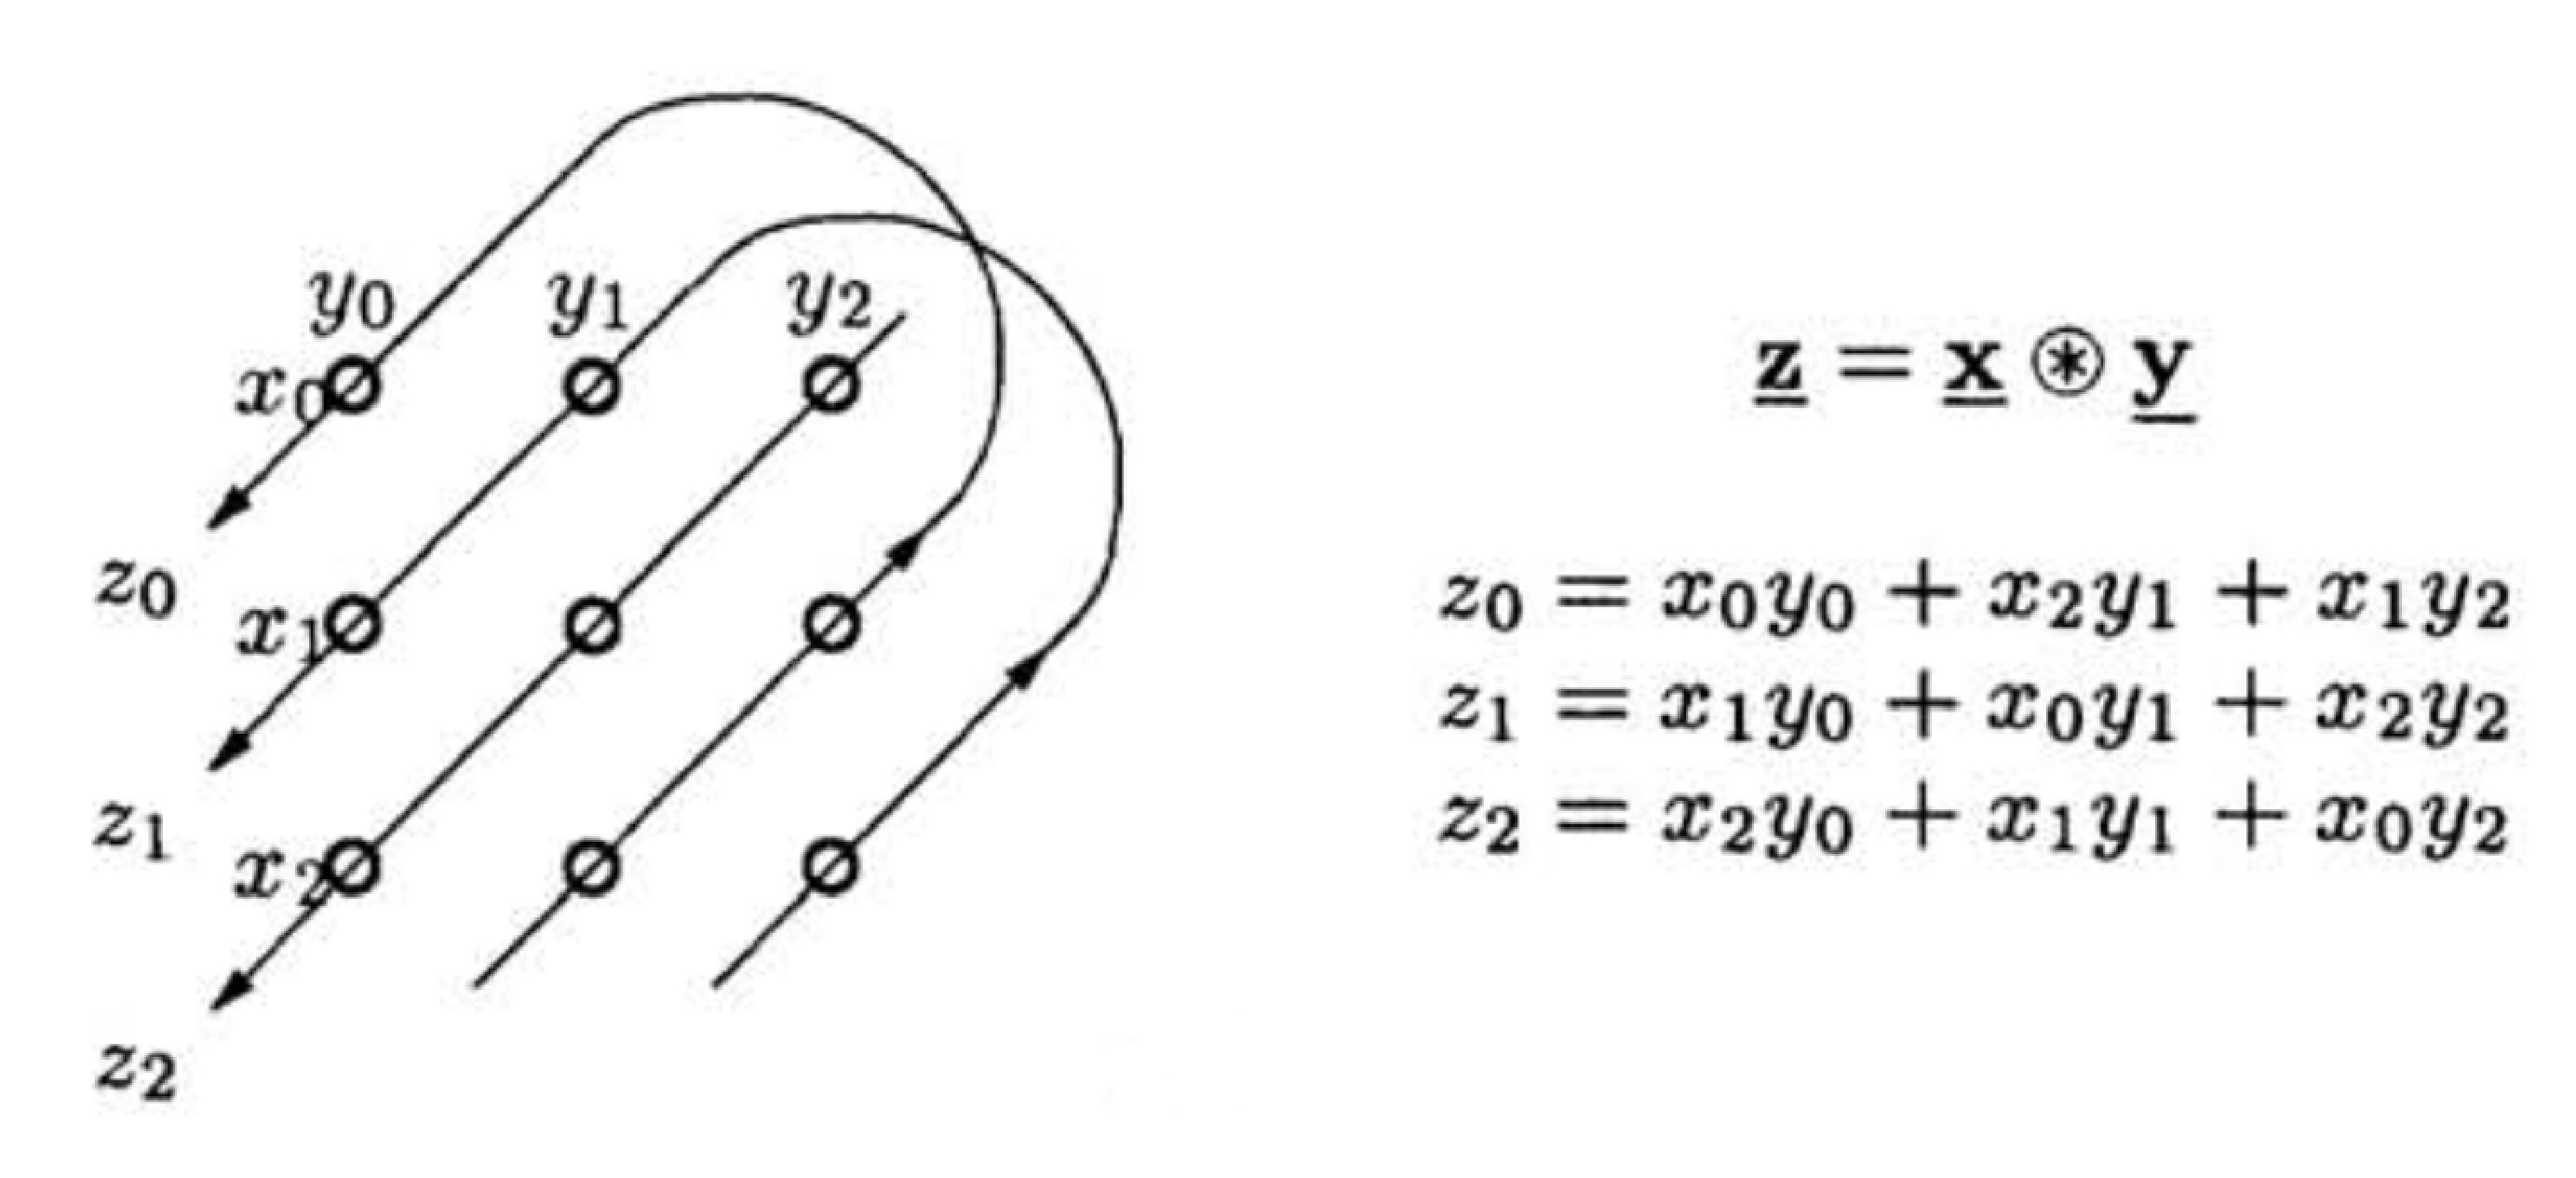
\includegraphics[width=0.85\textwidth]{imgs/circular_convolution_visualization_hor.eps}
			\caption{Visualization of circular convolution as compressed outer product for $3$-dimensional vectors. Image source \cite{Plate1994a}}
			\label{fig:circ_conv}
		\end{figure}
		The neutral element regarding circular convolution is $\pmb{1} = \left(1, 0, \cdots, 0\right)$.
		One important property of this operation is the fact, that circular convolution can efficiently be computed using the \ac{DFT}.
		The \ac{DFT} is defined as the function
        \begin{equation}
        \label{eq:dft}
		\abb{\ac{DFT}}{\mathbb{C}^{D}}{\mathbb{C}^{D}}{ \mathbf{x}}{\left(\sum_{j=0}^{D-1} x_{j} \zeta_{D}^{-jk} \right)_{k=0}^{D-1}} \qquad \textrm{ with } \zeta_{D} = \exp\left( \frac{i 2 \pi}{D} \right).
        \end{equation}
		Similarly, the \ac{IDFT} is defined as the function
        \begin{equation}
        \label{eq:inv_dft}
		\abb{\ac{IDFT}}{\mathbb{C}^{D}}{\mathbb{C}^{D}}{ \mathbf{x}}{\left( \frac{1}{D} \sum_{j=0}^{D-1} x_{j} \zeta_{D}^{jk} \right)_{k=0}^{D-1}}.
        \end{equation}
		From the convolution theorem \cite[Chap. 6]{Bracewell2000} we know, that we can calculate the circular convolution of any two vectors $ \mathbf{v}, \mathbf{w} \in V_{D}(N)$ by
        \begin{equation}
        \label{eq:conv_with_dft}
		\mathbf{v} \varoast \mathbf{w} = \ac{IDFT}\left(\ac{DFT}( \mathbf{v}) \odot \ac{DFT}( \mathbf{w}) \right),
        \end{equation}
		with $\odot$ denoting element-wise multiplication in this case.
		This induces that circular convolution obeys the same rules (commutativity and associativity) as element-wise multiplication, as both operations are the same except for a change of basis.
	\end{enumerate}
\end{ex}
As mentioned earlier, one of the most important features of (high-dimensional) \acp{VSA} is the fact that two random vectors are likely to be dissimilar.
We will derive this result in the following Theorem.
\begin{theorem}
	\label{theorem:VSA_cossim_distribution}
	Let $\left(V_{D}(N), \varoast, \oplus, \phi \right)$ a \acl{VSA}.
    For two randomly chosen vectors $ \mathbf{v}, \mathbf{w} \in V_{D}(N)$, the distribution of the similarity $\phi\left( \mathbf{v}, \mathbf{w}\right)$ is a version of the beta-distribution $\mathcal{B}_{\frac{D-1}{2},\frac{D-1}{2}}$ scaled and shifted to the interval $\left[-1,1\right]$ with mean $\mu=0$ and variance $\sigma^2=\frac{c^2}{D}$ up to a constant $c$.
    The standardized distribution trends towards a normal distribution with growing $D$.
\end{theorem}
\begin{proof}
	We will only give the proof of this Theorem for real valued \acp{VSA}, i.e., $N \subseteq \mathbb{R}$ and $\phi$ as the cosine similarity.
	Without loss of generality, we assume the vectors $ \mathbf{v}, \mathbf{w}$ picked randomly from the unit sphere $\mathbb{S}^{D-1} = \{ \mathbf{v} \in \mathbb{R}^{D} | \norm{ \mathbf{v}} = 1 \}$, as we can simply normalize the vectors by $\frac{ \mathbf{v}}{\norm{ \mathbf{v}}}$.
	Since binary \acp{VSA} can be associated with a euclidean sphere as well, the same result can be proven for those architectures with similar arguments (see \cite{Kanerva1988} for details).
	Due to symmetry of the unit sphere $\mathbb{S}^{D-1}$, we can furthermore - again without loss of generality - choose one vector as a unit vector, i.e., $ \mathbf{w}=\left(1, 0 , \cdots, 0\right)$.
	Thereby, the cosine similarity for $ \mathbf{v}=\left(v_{0}, \cdots, v_{D-1}\right)$ is given by $\phi\left( \mathbf{v}, \mathbf{w}\right) = v_{0}$
	By fixing one coordinate, we get the constraint $\sum_{i=1}^{D-1} v_{i}^{2} = 1-v_{0}^{2}$ which is equivalent to a lower dimensional sphere $\mathbb{S}^{D-2}$ with radius $\sqrt{1-v_{0}^2}$.
	Hence the cosine similarity $\phi\left( \mathbf{v}, \mathbf{w}\right)=:x$ is proportional to the surface of a conical frustum constructed from $\mathbb{S}^{D-2}$ with radius $\sqrt{1-x^{2}}$, slope $\frac{1}{\sqrt{1-x^{2}}}$ and some height $h$, i.e., the density function is proportional to
	\[
	f_{\phi( \mathbf{v}, \mathbf{w})}(x) \propto \frac{\sqrt{1-x^{2}}^{(D-2)}}{\sqrt{1-x^{2}}} h \propto \left(1-x^{2}\right)^{\frac{D-3}{2}}.
	\]
	Substituting $x=2u-1$, we get
	\[
	\left(1-\left(2u-1\right)^{2}\right)^{\frac{D-3}{2}} \propto \left(u-u^2\right)^{\frac{D-3}{2}} = \left(u \left(1-u\right)\right)^{\frac{D-3}{2}} = u^{\left(\frac{D-1}{2}-1\right)} \left(1-u\right)^{\left(\frac{D-1}{2}-1\right)},
	\]
	which is the density function of the beta distribution $\mathcal{B}_{\frac{D-1}{2},\frac{D-1}{2}}$.
	Thus, the cosine similarity is also beta distributed, but scaled and shifted to the interval $\left[-1,1\right]$ by $x=2u-1$.
    
	For $\alpha=\beta=\frac{D-1}{2}$, the mean of the beta distribution is $\tilde{\mu}=\frac{1}{2}$. Applying the substitution, we get the mean of the shifted distribution $\mu = 2\tilde{\mu }-1 = 0$.
    
	Making use of the simplification that the distribution of similarity is the same as the distribution in the first coordinate, the variance is given by the expected value of the square value of the first coordinate, i.e., $\mathbb{E}(v_{0}^{2})$.
	Since all coordinate are identically distributed, we get
	\[
	\mathbb{E}(v_{0}) = \frac{1}{D} \sum_{i=0}^{D-1} \mathbb{E}(v_{i}^2)= \frac{1}{D} \underbrace{\mathbb{E}\left(\sum_{i=0}^{D-1} v_{i}^2\right)}_{=:c^2}=\frac{c^2}{D}.
	\]
	Hence variance of the distribution of the cosine similarity is $\sigma^2=\frac{c^2}{D}$.
	In the particular case of the unit sphere $\mathbb{S}^{D-1}$, we get $c^{2}=1$ and a variance of $\sigma^2=\frac{1}{D}$.
    
	To see the convergence behavior of the standardized distribution, we look at the logarithm of its density function %$f_{\phi(v,w)}\left(\frac{x}{\sqrt{D}}\right)$
	\begin{equation}
	\label{eq:log_dens}
	\log\left(f_{\phi(v,w)}\left(\frac{x}{\sqrt{D}}\right)\right) = \frac{D-3}{2}\log\left(1-\frac{x^2}{D}\right) + C.
	\end{equation}
	Using the Taylor series approximation of the logarithm, equation~\eqref{eq:log_dens} transforms to
	\begin{align*}
		\log\left(f_{\phi(v,w)}\left(\frac{x}{\sqrt{D}}\right)\right) &= \frac{D-3}{2}\left(-\frac{x^2}{D} + \frac{x^4}{4D} \pm \ldots \right) + C = -\frac{1}{2}x^2 + \frac{3}{2D}x^2 + \mathcal{O}\left(\frac{x^4}{D}\right)  + C  \\
		&\longrightarrow -\frac{1}{2}x^2 + C = \log\left(f_{\mathcal{N}}\left(x\right)\right) \textrm{ for } D \longrightarrow \infty.
	\end{align*}
	Hence, with growing $D$ the standardized distribution of the cosine similarity trends to a normal distribution.
\end{proof}
Theorem~\ref{theorem:VSA_cossim_distribution} states, that the probability of finding two random, non-orthogonal vectors in a \ac{VSA} decreases with growing vector dimension.
\begin{figure}[t]
    \centering
    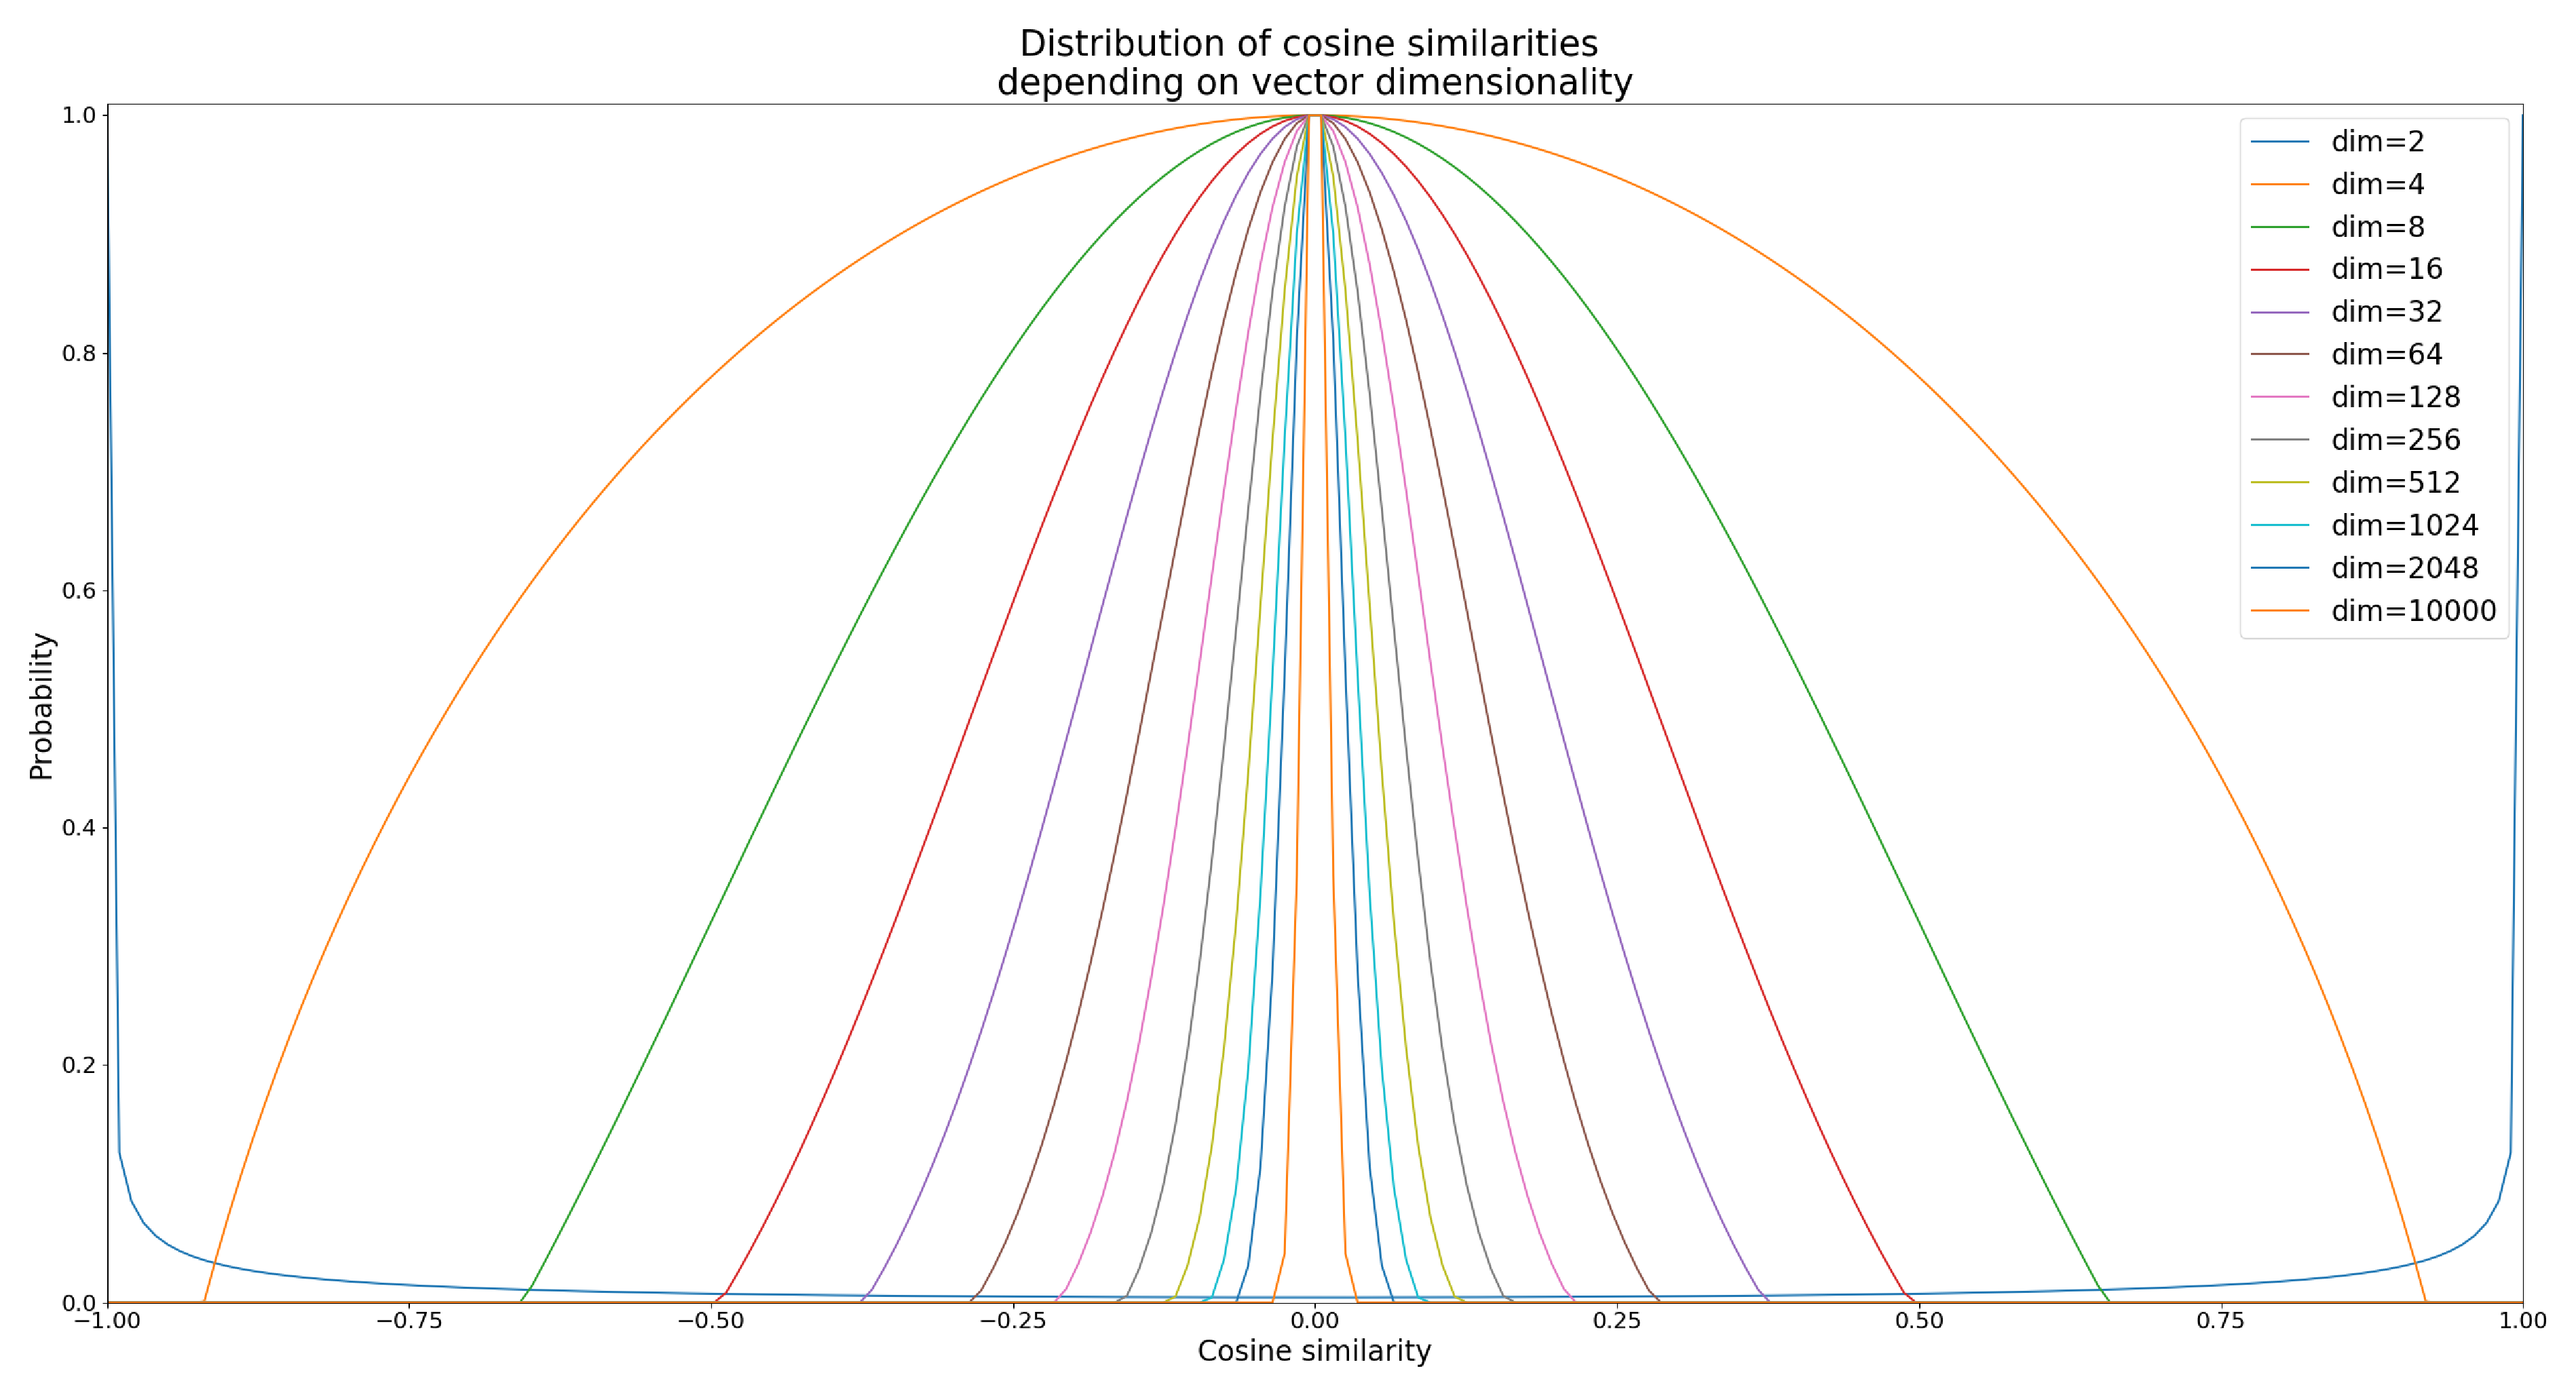
\includegraphics[width=1.\linewidth]{imgs/distributions_cosine_sims.eps}
    \caption{Visualization of the distribution of the cosine similarity between two randomly chosen vectors depending on their dimension.}
    \label{fig:distributions_cosine_sims}
\end{figure}
Figure~\ref{fig:distributions_cosine_sims}, which shows the probability distributions of cosine similarity for different vector dimensions, illustrates this result.
Furthermore, Theorem~\ref{theorem:VSA_cossim_distribution} allows us to give a more formal definition of the term "dissimilar".
\begin{defn}
	\label{def:similar}
	Let $(V_{D}(N), \varoast, \oplus, \phi)$ be a \acrfull{VSA} of dimension $D$ and $c \in \mathbb{N}$ a constant. We call any two vectors $ \mathbf{v}, \mathbf{w} \in v_{d}(n)$ \emph{dissimilar}, if
    \begin{equation}
    \label{eq:dissmilar}
	\left| \phi( \mathbf{v}, \mathbf{w}) \right| \leq \epsilon, \textrm{ with } \epsilon:=\tfrac{c}{\sqrt{D}}.
    \end{equation}
	Analogously, we call any two vectors $ \mathbf{v}, \mathbf{w} \in V_{D}(N)$ \emph{similar}, if	$\left| \phi( \mathbf{v}, \mathbf{w}) \right| > \epsilon$.
	Similar vectors are denoted by $ \mathbf{v} \approx \mathbf{w}$. 
\end{defn}
Definition~\ref{def:similar} can also be stated as follows: we consider any two vectors similar, if their similarity is higher than what we would expect from two randomly chosen vectors.
Therefore, we make use of the fact, that for growing dimension $D$, the cosine similarity follows approximately a normal distribution $\mathcal{N}_{\mu, \sigma}$, with $\mu=0$ and $\sigma=\tfrac{1}{\sqrt{D}}$ and the so-called three-sigma-rule.
This rule, which follows from Chebyshev's inequality, states that the probability $\mathbb{P}\left(\mu-3\sigma \leq X \leq \mu+3\sigma \right) \geq 0.95$ for any unimodal distributed random variable $X$.
For normally distributed $X$, we even have
\begin{align*}
	\mathbb{P}\left(\mu-2\sigma \leq X \leq \mu+2\sigma \right) &\approx 0.954 \\
	\mathbb{P}\left(\mu-3\sigma \leq X \leq \mu+3\sigma \right) &\approx 0.997.
\end{align*}
Given Definition~\ref{def:similar}, the probability of two randomly chosen vectors being similar is below \SI{5}{\percent} for $c=2$ and even below \SI{0.3}{\percent} for $c=3$, while the actual numerical interval $\left[-c\sigma, c\sigma\right]$ only depends on the vector dimension $D$.
Hence, we denote the weaker version of definition~\ref{def:similar} by $\epsilon_{weak} = \tfrac{2}{\sqrt{D}}$ as \emph{weak similarity threshold} and the stronger version by $\epsilon_{strong} = \tfrac{2}{\sqrt{D}}$ as \emph{strong similarity threshold}.
For lower \ac{VSA} dimensions such as $D \leq 50$, it can be beneficial to work with the weak similarity threshold, whereas for higher dimensions the stronger version can be used.

Based on the definition of similarity, we derive criteria for "good" multiplication functions in \acp{VSA}.
\begin{defn}
	\label{def:binding}
	Let $(V_{D}(N), \varoast, \oplus, \phi)$ be a \acrfull{VSA} of dimension $D$. We call its multiplication function
	\[\abb{\varoast}{V_{D}(N) \times V_{D}(N)}{K^{D}}{( \mathbf{v}, \mathbf{w})}{\varoast( \mathbf{v}, \mathbf{w}) =: \mathbf{v}\varoast \mathbf{w}}\]
	a \emph{binding function} if
	\begin{enumerate}
		\item for any two vectors $ \mathbf{v}, \mathbf{w} \in V_{D}(N)$, the vector $ \mathbf{v} \varoast \mathbf{w}$ is dissimilar to both $ \mathbf{v}$ and $ \mathbf{w}$, i.e.,
		\[
		\left| \phi( \mathbf{v}, \mathbf{v} \varoast \mathbf{w}) \right| \leq \epsilon \textrm{ and } \left| \phi( \mathbf{w}, \mathbf{v} \varoast \mathbf{w}) \right| \leq \epsilon.
		\]
		\item for any vector $ \mathbf{v} \in V_{D}(N)$, there exists a vector $\bar{\mathbf{v}} \in V_{D}(N)$ with $ \mathbf{v} \varoast \bar{\mathbf{v}} \approx \mathbf{1}$. We call $\bar{\mathbf{v}}$ a \emph{pseudo-inverse} element.
		If furthermore $ \mathbf{v} \varoast \bar{\mathbf{v}} = \mathbf{1}$, we call the vector $\bar{\mathbf{v}}$ \emph{exact inverse}.
	\end{enumerate}
\end{defn}
It is worth noting, that all multiplication operations mentioned in example~\ref{ex:VSAs} fulfill the criteria for binding functions as stated in Definition~\ref{def:binding}.
The first criteria is intended to allow structured representations in \acp{VSA}.
Representations built solely upon an addition function lack a mechanism to impose structure, as the sum of vectors is similar to all summands.
For continuous \acp{VSA}, this result is straightforward due to the linearity of the dot product, but it holds true for \acp{BSC} as well.
Therefore, summing vectors only allows to encode unordered sets of entities.
The property of binding functions to map two vectors to a vector dissimilar to both inputs enables structured representations.

The second criteria of Definition~\ref{def:binding} for binding functions is the basis to decode or recover the individual vector ingredients from structured representations.
The existence of a (pseudo-) inverse element allows the retrieval of $ \mathbf{v}, \mathbf{w} \in V_{D}(N)$ from $ \mathbf{v} \varoast \mathbf{w}$ by
\begin{equation}
\label{eq:retrieval}
\bar{\mathbf{v}} \varoast \left(\mathbf{v} \varoast \mathbf{w}\right) = \underbrace{\bar{\mathbf{v}} \varoast \mathbf{v}}_{\approx \mathbf{1}} \varoast \mathbf{w} = \tilde{\mathbf{w}} \approx \mathbf{w}.
\end{equation}
In case of exact inverse elements, the right hand side of equation~\eqref{eq:retrieval} becomes an exact equality $\tilde{\mathbf{w}}= \mathbf{w}$.
In most cases, however, the result $\tilde{\mathbf{w}}$ is not exactly equal to $ \mathbf{w}$, but similar.
It is this inherent inexactness of most \acp{VSA} what makes them suitable candidates for cognitive modeling \cite{Eliasmith2013}.
On the other hand, it imposes a functional demand for a clean-up memory.
A clean-up memory is a mechanism, which maps noisy versions of vectors like $\tilde{\mathbf{w}}$ to their exact counterparts, here $ \mathbf{w}$.
Therefore, we need to have a set of vectors, which represent established concepts or symbols the system has knowledge of.

\begin{defn}
	\label{def:clean-up-mem}
	Let $(V_{D}(N), \varoast, \oplus, \phi)$ be a \acrfull{VSA} of dimension $D$ with binding function $\varoast$.
	We call a finite subset $\vartheta \subsetneq V_{D}(N)$ a \emph{vocabulary}.
	A function $\abbil{\gamma}{K^{D}}{\vartheta}$ is called a \emph{clean-up memory}, if
	\begin{enumerate}
		\item for any vector $v\in K^{D}$ we have
		\[
		\phi\left( \mathbf{v}, \gamma(\mathbf{v})\right) > \phi\left( \mathbf{v}, \mathbf{w}\right), \textrm{ for any vector } \mathbf{w} \in \vartheta, \gamma( \mathbf{v}) \neq \mathbf{w}.
		\]
		\item for any two similar vectors $ \mathbf{v} \neq \tilde{\mathbf{v}} \in K^{D}, \mathbf{v} \in \vartheta$, i.e., $\tilde{\mathbf{v}} \approx \mathbf{v}$, we have $\gamma(\tilde{\mathbf{v}})= \mathbf{v}$.
	\end{enumerate}
\end{defn}
Definition~\ref{def:clean-up-mem} states, that the cleaned-up version of a vector is more similar to the original (noisy) version than any other vector in the vocabulary.

%----------------------------------------------------------------------------------------------------------
\section{The \acl{SPA}}
\label{sec:spa}
%----------------------------------------------------------------------------------------------------------

In this section, we focus on one particular \ac{VSA}, namely the \ac{SPA}, as we will be using it throughout this work.
The \ac{SPA} is an adoption of Plate's previously mentioned \acp{HRR} (cf.\ example~\ref{ex:VSAs}).
Revisiting definition~\ref{def:VSA}, the underlying number field of the \ac{SPA} is the field of real numbers, i.e., $N \subseteq \mathbb{R}$, the addition $\oplus$ and multiplication $\varoast$ operations are element-wise addition and circular convolution respectively, and the cosine similarity serves as measure of similarity $\phi$.
We will use $\mathcal{S}(D)$ as a short notation for the $D$-dimensional \ac{SPA} $(V_{D}(\mathbb{R}), \varoast, \oplus, \phi)$.
Eliasmith gives an in-depth description of the \ac{SPA} in \cite{Eliasmith2013}.
However, we recapitulate some important properties, which will be used later in this work.
\begin{figure}[t!]
	\centering
	\includegraphics[width=1.0\textwidth]{imgs/pseudo_inverse_tsplot_1.png}
	\caption{Visualization of the similarity $\phi\left(\mathbf{1}, v \varoast \bar{v}\right)$ between the neutral element $\mathbf{1}$ and the result of applying the pseudo-inverse to different vectors for varying vector dimensions. This plot shows the result of $100$ samples compared to the similarity threshold $\epsilon$.}
	\label{fig:pseudo_inv}
\end{figure}
\begin{lemma}
	\label{lemma:spa_pseudo_inv}
	Let $ \mathbf{v}=\left(v_0, \ldots, v_{D-1}\right)$ be an element of a $D$-dimensional \ac{SPA} $\mathcal{S}(D)$, i.e., $v_0, \ldots, v_{D-1} \in \mathbb{R}$.
	The vector $\bar{\mathbf{v}}=\left(v_0, v_{D-1}, \ldots, v_{1}\right)$ is a pseudo-inverse element of $ \mathbf{v}$ with respect to circular convolution, i.e., $ \mathbf{v} \varoast \bar{\mathbf{v}} \approx \mathbf{1}$.
\end{lemma}
Here, we skip an explicit proof for this lemma but rather point to \cite[Section 3.1.2 and 3.1.3]{Plate1994} for a in-depth derivation.
However, we visualize the similarity $\phi\left(\mathbf{1}, \mathbf{v} \varoast \bar{\mathbf{v}}\right)$ between the neutral element $\mathbf{1}$ and the result of applying the pseudo-inverse $ \mathbf{v} \varoast \bar{\mathbf{v}}$ compared to the similarity threshold $\epsilon$ (weak and strong version) in figure~\ref{fig:pseudo_inv}.
Therefore, we randomly chose \num{100} sample vectors for various dimensions, convolved them with their pseudo-inverse and compared the result to the neutral element $\mathbf{1}$.
We observe, that this similarity remains almost constant slightly above \num{0.7} and already for low vector dimensions ($D > 20$) way above the strong similarity threshold of $\epsilon=\frac{3}{\sqrt{D}}$.

Lemma~\ref{lemma:spa_pseudo_inv} states that we can find a pseudo-inverse element $\bar{\mathbf{v}}$ for any vector $ \mathbf{v}$ in a $D$-dimensional \ac{SPA} (given the dimension $D$ is sufficiently large).
Although we can also find an exact inverse element $ \mathbf{v}^{-1}$ for most vectors $ \mathbf{v}$, it is often more useful to work with pseudo-inverses instead of exact inverse elements.
We have already seen, that we can use the \acf{DFT} and \acf{IDFT} to calculate circular convolution efficiently by element-wise multiplication (this follows from the convolution theorem \cite[Chap. 6]{Bracewell2000}) in the frequency domain, i.e.,
\begin{equation}
    \mathbf{v} \varoast \mathbf{w} = \ac{IDFT}\left(\ac{DFT}( \mathbf{v}) \odot \ac{DFT}( \mathbf{w}) \right). \tag{\ref{eq:conv_with_dft} revisited}
\end{equation}
Furthermore, the \ac{DFT} of the convolutive neutral element $\mathbf{1} = \left(1, 0, \ldots, 0\right)$ is
\begin{equation}
	\ac{DFT}(\mathbf{1}) = \left(\exp\left(i0\right), \ldots, \exp\left(i0\right)\right) = \left(1, 1, \ldots, 1\right).
\end{equation}
This gives us a way of finding an exact inverse element $ \mathbf{v}^{-1}$ by
\begin{equation}
	\ac{DFT}(\mathbf{1}) = \ac{DFT}( \mathbf{v}) \odot \ac{DFT}( \mathbf{v}^{-1}).
\end{equation}
By denoting the $j$-th element of the Fourier Vector $\ac{DFT}( \mathbf{v})$ with $\ac{DFT}_{j}( \mathbf{v})$, we get
\begin{equation}
\label{eq:inv_elemtwise_fourier}
	\ac{DFT}_{j}( \mathbf{v}) \odot \ac{DFT}_{j}( \mathbf{v}^{-1}) = 1 \quad \textrm{ for } j \in \left\{0, \ldots, D-1\right\}.
\end{equation}
If we express $\ac{DFT}_{j}( \mathbf{v}) \in \mathbb{C}$ in polar coordinates, i.e., $\ac{DFT}_{j}( \mathbf{v}) = r_j \exp\left(i\varphi_j\right)$, we directly get from equation~\eqref{eq:inv_elemtwise_fourier} that $\ac{DFT}_{j}( \mathbf{v}^{-1}) = \frac{1}{r_j} \exp\left(-i\varphi_j\right)$.
By using the symmetry property of the real-valued \ac{DFT}, we can see that the transform $\ac{DFT}_j(\bar{\mathbf{v}})$ of the pseudo-inverse element $\bar{\mathbf{v}}$ from Lemma~\ref{lemma:spa_pseudo_inv} is the complex conjugate of $\ac{DFT}_j( \mathbf{v})$, i.e., we can write $\ac{DFT}_j(\bar{\mathbf{v}}) = r_j \exp\left(-i\varphi\right)$ in polar coordinates.
From those equations, we can see that the pseudo-inverse $\bar{\mathbf{v}}$ has the same norm as the original vector $ \mathbf{v}$, i.e., $\norm{ \mathbf{v}} = \norm{\bar{\mathbf{v}}}$, whereas the norm of the exact inverse $ \mathbf{v}^{-1}$ can become significantly larger than the norm of $ \mathbf{v}$ in some cases.
This is due to the fact, that elements of the transform of the pseudo-inverse have the same lengths $r_j$ as the original vector, whereas the transformed elements of the exact inverse have lengths $\frac{1}{r_j}$, which can become significantly large when $r_j$ is close to $0$.
The relation between the vector norm and the magnitudes in the frequency domain is given by Parseval's theorem (also known as Rayleigh's theorem) \cite[Chap. 6]{Bracewell2000}, which states
\begin{equation}
\label{eq:parseval}
\norm{\mathbf{v}}^2 = \sum_{k=0}^{D-1} \left| v_{k} \right|^{2} = \frac{1}{D} \sum_{k=0}^{D-1} \left|\ac{DFT}_{k}\left( \mathbf{v}\right)\right|^{2} = \sum_{k=0}^{D-1} r_{k}^{2}.
\end{equation}
This can lead to additional noise when retrieving vectors from structured representations (cf.\ equation~\eqref{eq:retrieval}).
However, there is a certain class of vectors, for which the pseudo- and exact inverse element coincide.
\begin{defn}
	\label{def:unitary_vec}
	Let $ \mathbf{v}$ be a vector in a $D$-dimensional \ac{SPA} $\mathcal{S}(D)$ with exact and pseudo-inverse elements $ \mathbf{v}^{-1}$ and $\bar{\mathbf{v}}$ respectively.
	We call $ \mathbf{v}$ a \emph{unitary vector}, if and only if $ \mathbf{v}^{-1} = \bar{\mathbf{v}}$.
	We denote the set of unitary vectors by $\mathcal{U} \subset \mathcal{S}(D)$.
\end{defn}
\begin{defn}
	\label{def:conv_power}
	Let $ \mathbf{v}$ be a vector in a $D$-dimensional \ac{SPA} $\mathcal{S}(D)$. We define the \emph{convolutive power} by an exponent $p \in \mathbb{R}$ by
	\[
	\mathbf{v}^{p} := \Re\left(\ac{IDFT} \left(\left(\ac{DFT}_{j}\left( \mathbf{v}\right)^{p}\right)_{j=0}^{D-1}\right)\right),
	\]
	where $\Re$ denotes the real part $a$ of a complex number $a + ib \in \mathbb{C}$.
\end{defn}
Unitary vectors take a special role in the \ac{SPA} as they have some interesting and useful properties.
\begin{lemma}
	\label{lemma:unitary_vec}
	Let $\mathcal{U}$ be the set of unitary vectors in the $D$-dimensional \ac{SPA} $\mathcal{S}(D)$.
    The following statements hold
 	\begin{enumerate}[label=\roman*]
		\item All elements of $\mathcal{U}$ have unit length, i.e., we have $\norm{\mathbf{u}} = 1$ for any vector $ \mathbf{u} \in \mathcal{U}$.
		\item $\mathcal{U}$ is closed under convolutive exponentiation, i.e., $ \mathbf{u}^{p} \in \mathcal{U}$ for any $ \mathbf{u} \in \mathcal{U}$ and $p \in \mathbb{R}$.
        \item The product under circular convolution of two unitary vectors is unitary, i.e.\ $ \mathbf{u}_{1} \varoast \mathbf{u}_{2} \in \mathcal{U} $ for $ \mathbf{u}_{1}, \mathbf{u}_{2} \in mathcal{U}.$
		\item Convolution with unitary vectors preserves the norm, i.e., $\norm{\mathbf{v}} = \norm{ \mathbf{v} \varoast \mathbf{u}}$ for any $ \mathbf{v} \in \mathcal{S}(D), \mathbf{u} \in \mathcal{U}$.
	\end{enumerate}
\end{lemma}
\begin{proof}
	To show, that unitary vectors have unit length, we directly calculate the first component of convolution $ \mathbf{z} := \mathbf{u} \varoast \bar{ \mathbf{u}}$ between a unitary vector $ \mathbf{u}$ and its pseudo-inverse $\bar{ \mathbf{u}}$:
	\[
	z_{0} = \sum_{k=0}^{D-1} u_{k} \bar{u}_{-k \Mod{D}} = \sum_{k=0}^{D-1} u_{k}^{2} = \norm{ \mathbf{u}}^{2}.
	\]
	As $ \mathbf{u}$ is a unitary vector, we have $ \mathbf{u}^{-1} = \bar{ \mathbf{u}}$ and therefore $ \mathbf{u}\varoast \bar{ \mathbf{u}} = \mathbf{1}$.
	Thus, we have for the first component of $ \mathbf{z} := \mathbf{u} \varoast \bar{ \mathbf{u}}$
	\[
	1 = z_{0} = \norm{ \mathbf{u}}^{2},
	\]
	which gives the first result of the lemma.
    
	To show that the set of unitary vectors $\mathcal{U}$ is closed under convolutive exponentiation, we write each component of $\ac{DFT}( \mathbf{u})$ for $ \mathbf{u} \in \mathcal{U}$ in polar coordinates, i.e., $\ac{DFT}_j( \mathbf{u}) = r_j\exp\left(\varphi_j\right)$.
	From previous considerations, we know that $\ac{DFT}_j( \mathbf{u}^{-1}) = \frac{1}{r_j}\exp\left(-\varphi_j\right)$ and $\ac{DFT}_j(\bar{ \mathbf{u}}) = r_j\exp\left(-\varphi_j\right)$, which gives $r_j=1$ for $j=0, \ldots, D-1$ because $ \mathbf{u}$ is a unitary vector.
	Thus, we have for any $p \in \mathbb{R}$
	\[
	\ac{DFT}_j\left( \mathbf{u}^{p}\right) = \ac{DFT}_j\left( \mathbf{u}\right)^{p} = r_j^{p}\exp\left(ip\varphi\right) = 1^{p} \cdot \exp\left(ip\varphi\right),
	\]
	which makes $ \mathbf{u}^{p}$ itself a unitary vector, as all magnitudes are $1$.	

    Similarly, we proof that the convolution of two unitary vectors is again unitary. 
    Let $ \mathbf{u}_{1}, \mathbf{u}_{2} \in \mathcal{U}$ be unitary vectors, then we have
    \[
        \ac{DFT} \left( \mathbf{u}_1 \varoast \mathbf{u}_2\right) = \ac{DFT} \left( \ac{IDFT} \left( \ac{DFT} \left( \mathbf{u}_1\right) \odot \ac{DFT} \left( \mathbf{u}_2\right)\right)\right) =  \ac{DFT} \left( \mathbf{u}_1\right) \odot \ac{DFT} \left( \mathbf{u}_2\right).
    \]
    Writing both $\ac{DFT}_j( \mathbf{u}_1) = r_{1j}\exp\left(\varphi_{1j}\right)$ and $\ac{DFT}_j( \mathbf{u}_2) = r_{2j}\exp\left(\varphi_{2j}\right)$ in polar coordinates, we get 
    \[
        \ac{DFT}_j \left( \mathbf{u}_1 \varoast \mathbf{u}_2\right) = r_{1j} \cdot r_{2j} \cdot \exp \left(\varphi_{1j} + \varphi_{2j}\right) = 1 \cdot \exp \left(\varphi_{1j} + \varphi_{2j}\right),
    \]
    as we have $r_{1j}=1$ and $r_{2j}=1$ for all magnitudes since both $ \mathbf{u}_1$ and $ \mathbf{u}_2$ are unitary vectors.
    This in turn makes their product under convolution unitary as well.
    
    To proof that convolution with unitary vectors preserves the norm, we use Parseval's theorem (cf.\ equation~\eqref{eq:parseval}) again.
	For any vector $ \mathbf{v} \in \mathcal{S}(d)$ and  a unitary vector $ \mathbf{u} \in \mathcal{U}$, we denote $ \mathbf{z}:=  \mathbf{v} \varoast \mathbf{u}$ and get
	\begin{equation}
	\label{eq:norm_parseval}
	\norm{ \mathbf{v} \varoast \mathbf{u}}^{2} = \sum_{k=0}^{D-1} \left|z_{k}\right|^{2} = \frac{1}{D} \sum_{k=0}^{D-1} \left|\ac{DFT}_{k}( \mathbf{z})\right|^{2} = \frac{1}{D} \sum_{k=0}^{D-1} \left|\ac{DFT}_{k}( \mathbf{v}) \cdot \ac{DFT}_{k}( \mathbf{u})\right|^{2}.
	\end{equation}
	Writing $\ac{DFT}_{k}( \mathbf{v}) = r_{vk}\exp\left(i\varphi_{vk}\right)$ and $\ac{DFT}_{k}( \mathbf{u}) = r_{uk}\exp\left(i\varphi_{uk}\right)$ in polar coordinates with $r_{uk} = 1$ for $k=0, \ldots, D-1$ as $u$ is unitary, equation~\eqref{eq:norm_parseval} transforms to
	\begin{equation*}
	\norm{ \mathbf{v} \varoast \mathbf{u}}^{2} = \frac{1}{D} \sum_{k=0}^{D-1} \left|r_{vk} \exp\left(i\left(\varphi_{vk} + \varphi_{uk}\right)\right)\right|^{2} = \frac{1}{D} \sum_{k=0}^{D-1} \left|r_{vk}\right|^{2} = \frac{1}{D} \sum_{k=0}^{D-1} \left|\ac{DFT}_k\left( \mathbf{v}\right)\right|^{2} = \norm{ \mathbf{v}}^{2}.
	\end{equation*}
\end{proof}

%----------------------------------------------------------------------------------------------------------
\section{The \acl{NEF}}
\label{sec:neural_eng}
%----------------------------------------------------------------------------------------------------------

In this section, we make a short excursion and give a brief overview of the \acf{NEF}, as we will be making use of it in forthcoming chapters.
The \ac{NEF} \cite{Eliasmith2003} is a mathematical theory, which provides a set of methods to construct biologically plausible, large-scale neural models.
These methods can be divided into the three main principles of the \ac{NEF}: \emph{representation}, \emph{transformation} and \emph{dynamics}.
The \ac{Nengo} \cite{Bekolay2014, Nengo} software suite is a python library, which implements the \ac{NEF}'s principles.
\ac{Nengo} has been used to build a variety of neural models, e.g.\ models of the basal ganglia system \cite{Stewart2010, Stewart2012} and \acf{Spaun} \cite{Eliasmith2012}, a large-scale, functional model of the brain, which is able to perform eight cognitive tasks.
Furthermore, \ac{Nengo} has been used to interface neural models with physical, neuromorphic hardware systems and robots \cite{Conradt2014, Stewart2016, Mirus2018a}.
Here, we give a brief introduction to the \ac{NEF}'s principles and refer to \cite{Eliasmith2003, Eliasmith2013, Bekolay2014} for more details.
\subsection{Representation}
\label{subsec:nef_representation}
The first principle of the \ac{NEF}, representation, provides mathematical tools to encode information, namely time-varying real-valued vectors, in the activity of neural populations.
It is based on the assumption, that neurons have a "preferred direction vector" in the represented space, each neuron responds most strongly to.
This assumption is grounded by the findings of \cite{Georgopoulos1989} that each neuron in motor cortex of rhesus monkeys has a different preferred arm direction.
The \ac{NEF} expands this idea to neural representations in general.
\begin{figure}[t!]
	\centering
	\subfloat[Tuning curves \label{subfig:nef_rep_tuning_curves}]{%
		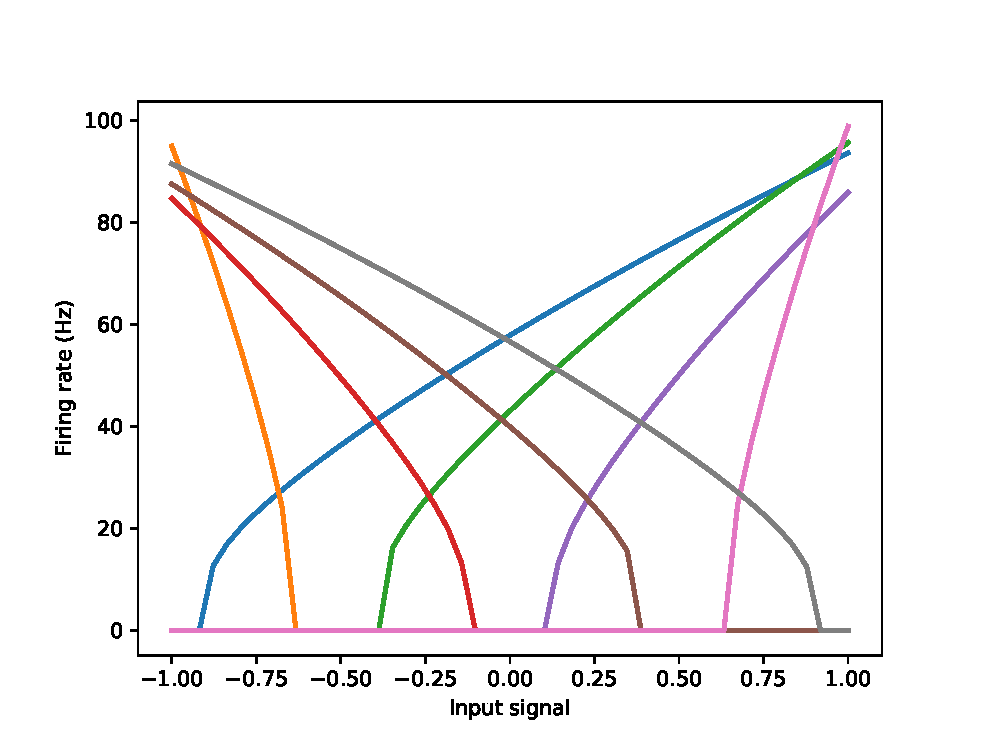
\includegraphics[width=0.45\textwidth]{imgs/NEF_tuning_curves.eps}
	}
	\subfloat[Spike times\label{subfig:nef_rep_spike_raster}]{%
		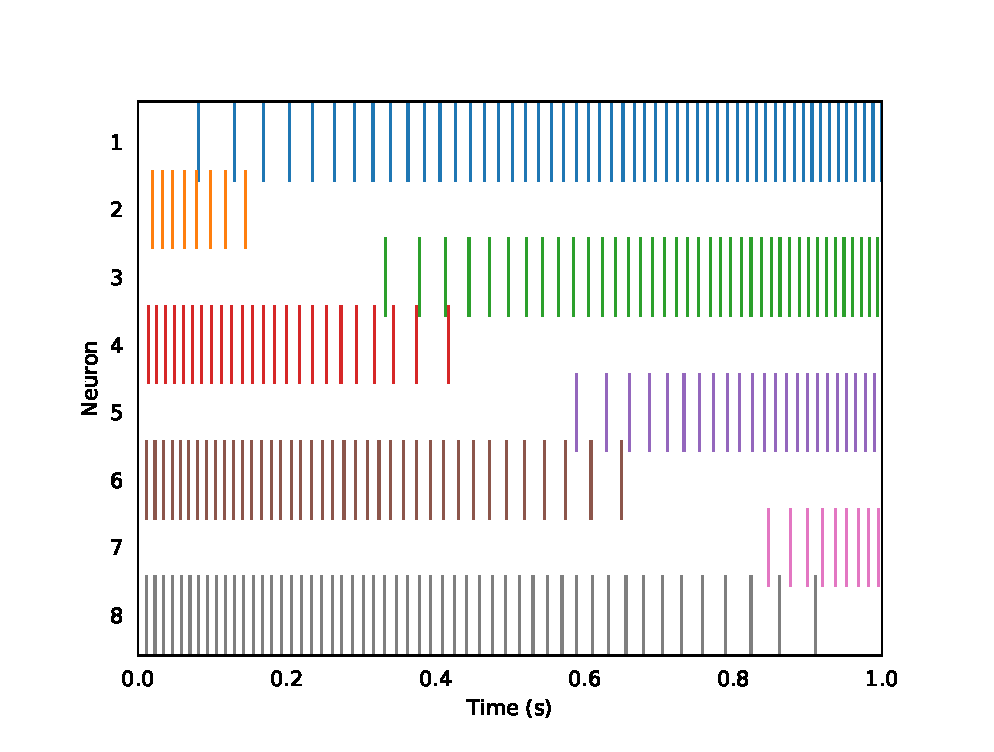
\includegraphics[width=0.45\textwidth]{imgs/NEF_spikes_raster.eps}
	}\\
	\vspace{-0.4cm}
	\subfloat[Decoded output\label{subfig:nef_rep_decoded}]{%
		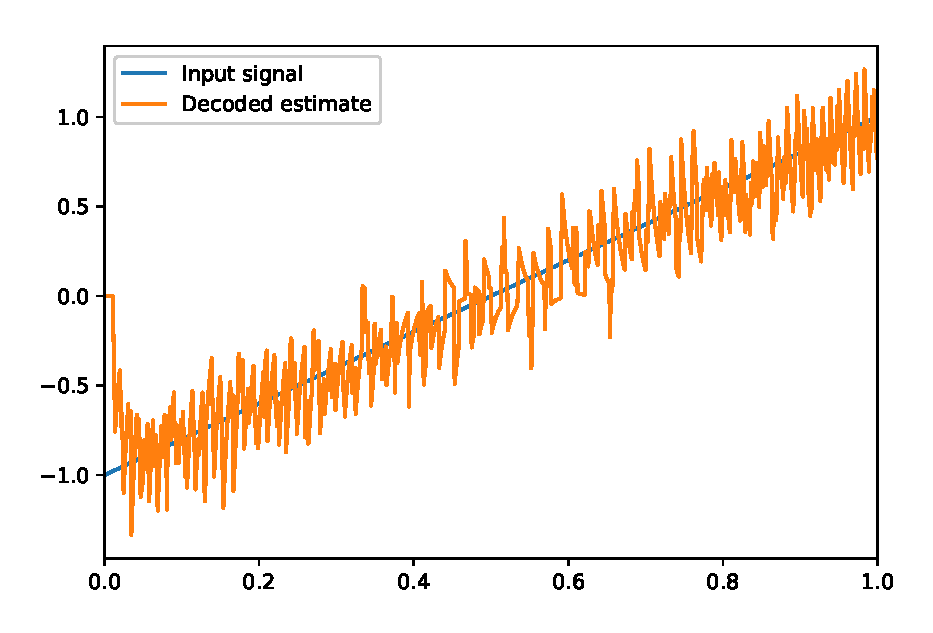
\includegraphics[width=0.45\textwidth]{imgs/NEF_decoded_output.eps}
	}
	\subfloat[Filtered neural activity\label{subfig:nef_rep_spike_filtered}]{%
		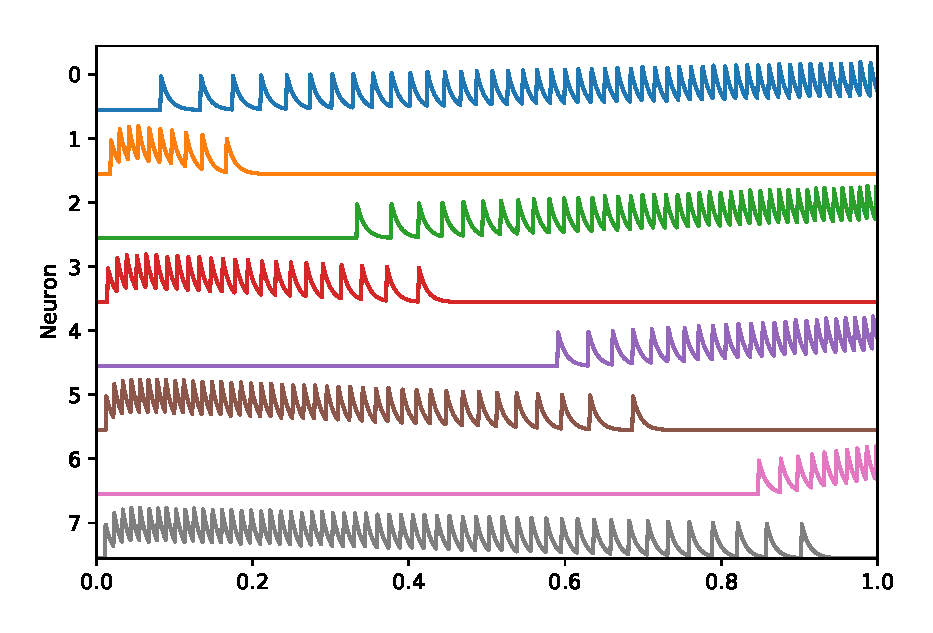
\includegraphics[width=0.45\textwidth]{imgs/NEF_spikes_filtered.eps}
	}
	\caption{The representation principle of the \ac{NEF}. Images adapted from \cite{Bekolay2014}}\label{fig:nef_representation}
\end{figure}
Let $A$ be a population of $N \in \mathbb{N}$ neurons encoding a subset $V$ of a real-valued vector space, i.e., $V\subseteq \mathbb{R}^{n}$.
Given a function $\abbil{\mathbf{x}}{\mathbb{R}}{V}$, we can write the activity $a_{i}$ of the $i$-th neuron in a neural population encoding a time-varying vector $\mathbf{x}(t)$ as a spike train, i.e., a sum of delta functions
\begin{equation}
a_{i}\left(\mathbf{x}(t)\right) = \sum_{j=1}^{m_{i}} \delta(t - t_{j}) = G_{i}(\underbrace{\alpha_{i}\langle\mathbf{e}_{i},\mathbf{x}(t)\rangle + J_{i}}_{=:c}) \quad \textrm{ for } 1 \leq i \leq N,
\label{eq:nef_encoding}
\end{equation}
where $G_{i}$ is the spiking neural non-linearity, $\alpha_{i}$ is the gain of the neuron, $\mathbf{e}_{i}$ is the neuron's preferred direction or encoding vector and $J_{i}$ is a bias current to account for neural background activity and $t_{j}$ are the $m_{i}$ spike-times of the $i$-th neuron.
Notably, the current flowing into the cell is completely determined by $c$, whereas the spiking behavior of the neuron model is represented by the non-linear function $G_{i}$.
The input current $c$ and therefore the \ac{NEF}'s encoding process is independent of particular spiking neuron models.

To decode the input values $\mathbf{x}(t)$ back out of the neural population $A$, the spike train is convolved with an exponentially decaying filter $\abbil{h}{\mathbb{R}}{\mathbb{R}}$ to simulate the process of neurons generating post-synaptic current after spiking (cf.\ figure~\ref{subfig:nef_rep_spike_filtered}) resulting in
\begin{equation}
\tilde{a}_{i}\left(\mathbf{x}(t)\right) = \sum_{j=1}^{m_{i}} h(t) \ast \delta(t - t_{j}) = \sum_{j=1}^{m_{i}} h(t - t_{j}).
\label{eq:nef_filtered_activity}
\end{equation}
A simple model of an exponential decaying filter is the function $\abb{h}{\mathbb{R}}{\mathbb{R}}{t}{e^{\sfrac{-t}{\tau_{p}}}}$, where $\tau_{P}$ denotes the post-synaptic time constant.
We obtain an estimation $\mathbf{\hat{x}}(t)$ of the original input $\mathbf{x}(t)$ as a weighted sum with some decoder values $\mathbf{d}_{i}$
\begin{equation}
\mathbf{\hat{x}}(t) = \sum_{i=1}^{N} \tilde{a}_{i}\left(\mathbf{x}(t)\right) \mathbf{d}_{i}.
\label{eq:nef_decoding}
\end{equation}
To calculate the optimal decoders $\mathbf{d}_{i}$, we need to minimize the error between input $\mathbf{x}(t)$ and decoded output $\mathbf{\hat{x}}(t)$
\begin{equation}
E = \int \left( \mathbf{x}(t) - \sum_{i=1}^{N} \tilde{a}_{i}\left(\mathbf{x}(t)\right) \mathbf{d}_{i}\right)^{2} \diff \mathbf{x}(t).
\label{eq:decoder_calculation}
\end{equation}
\ac{Nengo} solves for the decoders $\mathbf{d}_{i}$ by default using least squares optimization \cite{Eliasmith2013}[Appendix B1].
Figure~\ref{fig:nef_representation} visualizes this encoding process for $V = \left[ -1, 1\right] \subset \mathbb{R}$ and a population of $8$ neurons.
Figure~\ref{subfig:nef_rep_tuning_curves} shows the tuning curves of individual neurons, which define how these neurons respond to specific input values.
Equation~\eqref{eq:nef_encoding} is depicted in figure~\ref{subfig:nef_rep_spike_raster}, which shows a raster plot of the neurons' spike times based on the input signal shown in figure~\ref{subfig:nef_rep_decoded}.
Figure~\ref{subfig:nef_rep_spike_filtered}, which shows the filtered neural activity for each neuron, visualizes equation~\eqref{eq:nef_filtered_activity}.
Finally, figure~\ref{subfig:nef_rep_decoded} depicts the original input value as well as the estimated output of the neural populations' activity (cf.\ equation~\eqref{eq:nef_decoding}).
Note, that the neural population's decoded output is only a noisy approximation of the original input value, whose accuracy can be improved by increasing the number of neurons in the population.
\subsection{Transformation}
\begin{figure}[t]
	\centering
	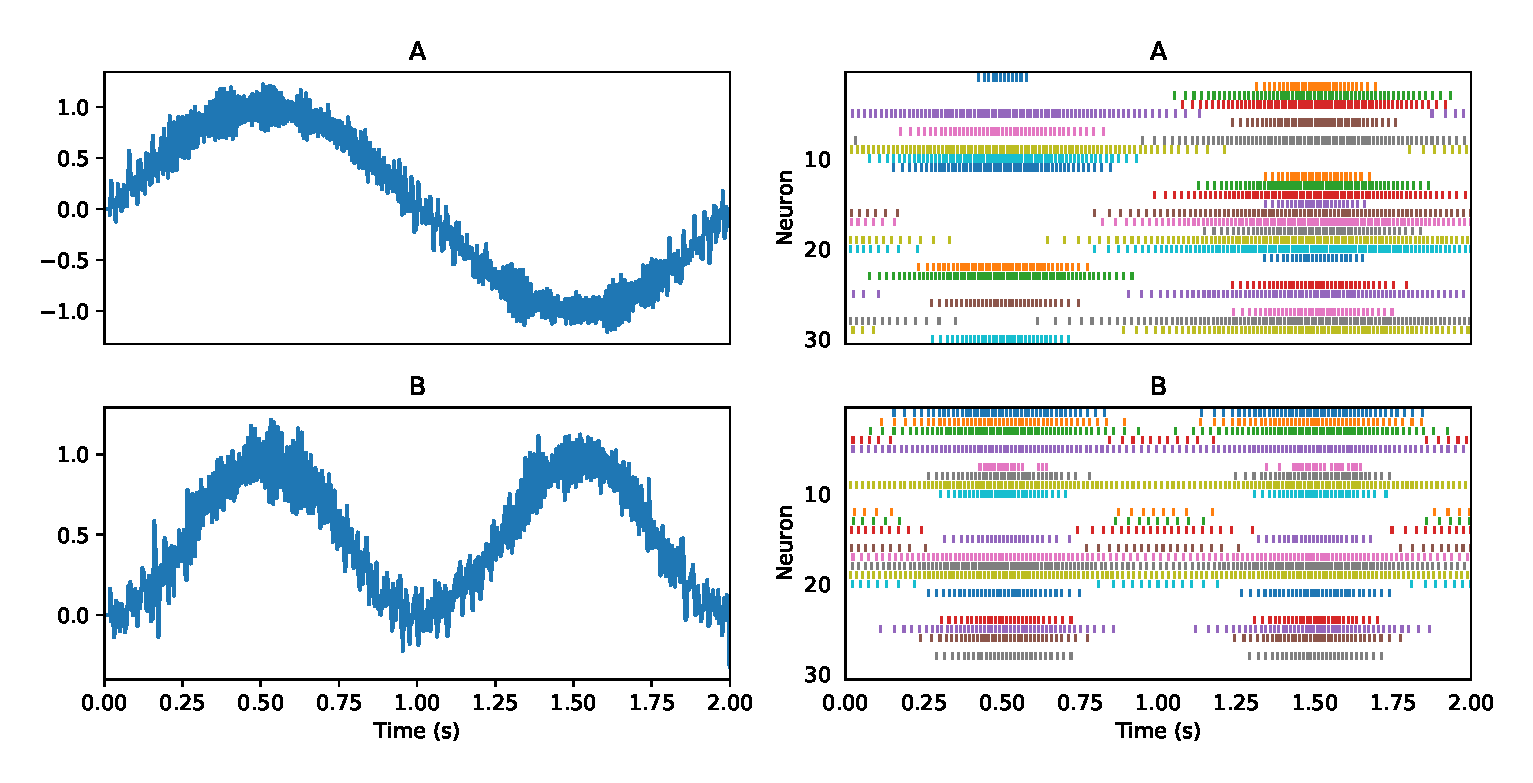
\includegraphics[width=0.85\textwidth]{imgs/NEF_transformation.eps}
	\caption{The transformation principle of the \ac{NEF}.
    Images adapted from \cite{Nengo}.}
	\label{fig:nef_transformation}
\end{figure}
The second main principle of the \ac{NEF}, \emph{transformation}, provides the mathematical tools to compute functions across connections between populations of neurons.
Let $A$ resp. $B$ be populations of $N$ resp. $M$ neurons encoding a time-varying vector $\mathbf{x}(t) \in V \subset \mathbb{R}^{n}$ resp. $\mathbf{y}(t) \in W \subset \mathbb{R}^{m}$ according to the representation principle and a function $\abbil{f}{V}{W \subset \mathbb{R}^{m}}$.
In order to approximate the function $f$ across a connection from population $A$ to population $B$, we use the tools of the representation principle, but we calculate a different set of decoder values $\mathbf{d}_{i}^{f}$ for population $A$ by minimizing the error
\begin{equation}
\label{eq:nef_transformation}
E = \int \left( f(\mathbf{x}(t)) - \sum_{i=1}^{N} \tilde{a}_{i}\left(\mathbf{x}(t)\right) \mathbf{d}_{i}^{f}\right)^{2} \diff \mathbf{x}(t).
\end{equation}
Given encoders $\mathbf{e}_{j}^{B}$ and gain $\alpha_{j}^{B}$ for $1 \leq j \leq M$ of population $B$, we can derive a weight matrix for the connection from $A$ to $B$ approximating the function $f$ by
\begin{equation}
w_{ij} = \alpha_{j}^{B} \mathbf{d}_{i}^{f} L \mathbf{e}_{j}^{B} \quad \textrm{for } 1 \leq i \leq N \textrm{ and } 1 \leq j \leq M,
\end{equation}
where $L$ is a $M \times N$ linear operator.
Here, the \ac{NEF} makes the assumption, that connection weights can be factored into encoders, decoders and a linear transform.
Figure~\ref{fig:nef_transformation} visualizes this \ac{NEF}'s transformation principle for $V = W = \left[ -1, 1\right] \subset \mathbb{R}$, two neural populations $A$, $B$ containing $30$ neurons each.
The left and right panel of plots shows the populations' decoded outputs and the neurons' spike times respectively.
Population $A$ uses the representation principle to encode a sine function, whereas the transformation principle was used to calculate the function $\abb{f}{V}{W}{x}{f(x)=x^{2}}$ across the connection from $A$ to $B$.

\subsection{Dynamics}

\begin{figure}[t]
	\centering
\begin{tikzpicture}[%
auto,
%scale=3,
block/.style={
	rectangle,
	draw=blue,
	thick,
	fill=blue!20,
	text width=3em,
	align=center,
	rounded corners,
	minimum height=4em,
},
circ/.style={
	circle,
	draw=orange,
	thick,
	fill=orange!20,
	text width=3em,
	align=center,
	rounded corners,
	minimum height=6em,
}
]
\node[block] (X) at (1,1) {\Huge $\mathbf{x}$};
\node[circ] (A) [right=2cm of X] {\Huge  $A$ \\ \vspace{0.5em} \Large $\ast h(t)$};
\node[block] (Y) [right=2cm of A] {\Huge $\mathbf{y}$};
\draw [thick,->] (X) -- (A) node [midway, below] {\Large $f\left(\mathbf{x}\left(t\right)\right)$};
\draw [thick,->] (A) -- (Y);
% Calculate branch point coordinates
\path (A) -- coordinate (branch) (Y);
\path (X) -- coordinate (branch_end) (A);
\coordinate[above=2cm of branch] (branch_ab);
\coordinate[above=2cm of branch_end] (branch_end_ab);
\draw [thick,->] (branch) -- (branch_ab) -- (branch_end_ab) node [midway, above] {\Large $g\left(\mathbf{y}\left(t\right)\right)$} -- (branch_end);
\end{tikzpicture}
\caption{The dynamics principle of the \ac{NEF} for recurrent connections.}
\label{fig:nef_dynamics}
\end{figure}
\todo[inline]{check if figure~\ref{fig:nef_dynamics} can be beautified}
The third main principle of the \ac{NEF}, \emph{dynamics}, provides a set of mathematical tools to implement dynamical systems in neural populations through recurrent connections.
Let $A$ be a population of neurons with an incoming connection approximating the function $\abbil{f}{V}{W \subset \mathbb{R}^{m}}$ and a recurrent connection approximating the function $\abbil{g}{W}{W}$ (cf.\ figure~\ref{fig:nef_dynamics}).
Thus, the overall function the population is approximating is
\begin{equation}
\mathbf{y}(t) = h(t) \ast \left(f(\mathbf{x}(t)) + g(\mathbf{y}(t))\right)
\label{eq:nef_dyn}
\end{equation}
with exponential decaying filter function $\abb{h}{\mathbb{R}}{\mathbb{R}}{t}{e^{\sfrac{-t}{\tau}}}$.
By applying the Laplace transform to equation~\eqref{eq:nef_dyn}, we get
\begin{equation}
\label{eq:nef_dyn_laplace}
\mathbf{Y}(s) = \frac{1}{1 + s\tau}\left(F(\mathbf{X}(s)) + G(\mathbf{Y}(s))\right).
\end{equation}
We can rearrange equation~\eqref{eq:nef_dyn_laplace} to
\begin{equation}
s\mathbf{Y}(s) = \frac{G(\mathbf{Y}(s))-\mathbf{Y}(s)}{\tau} + \frac{F(\mathbf{X}(s))}{\tau}.
\end{equation}
Transforming back leads to the differential equation
\begin{equation}
\frac{\partial \mathbf{y}(t)}{\partial t} = \frac{g(\mathbf{y}(t)-y)}{\tau} + \frac{f(\mathbf{x}(t))}{\tau}.
\end{equation}
Thus, to construct a neural model approximating a differential equation of the form
\begin{equation}
\frac{\mathbf{y}(t)}{\partial t} = a(\mathbf{y}(t)) + b(\mathbf{x}(t))
\label{eq:nef_dyn_diffeq}
\end{equation}
with functions $\abbil{a}{W}{W}$ and $\abbil{b}{V}{W}$, the first two principles of the \ac{NEF} can be used to create a neural population of the form as shown in figure~\ref{fig:nef_dynamics}.
By setting the functions $g(\mathbf{y}(t))=\tau a(\mathbf{y}(t)) + \mathbf{y}(t)$ and $f(\mathbf{x}(t))=\tau b(\mathbf{x}(t))$, we obtain a neural model approximating the desired dynamical system described by the differential equation~\eqref{eq:nef_dyn_diffeq}.

\section{Cognitive Modeling with \aclp{VSA}}%
\label{sec:cognitive_modelling_with_vsa}

In this section, we give a brief introduction of how we can use the theory shown in sections~\ref{sec:math_prop_vsas} and~\ref{sec:spa} to represent (structured) information using \acp{VSA}.
We give a general overview of different ways to establish vocabularies containing atomic vectors and how we can build more complex representations from those elementary ingredients.
The authors of \cite{Gallant2013} refer to these two steps as the first two of three stages for generating structured vector representations: the \emph{pre-processing stage} (generating a vocabulary; see also section~\ref{sec:preprocessing_stage_generating_a_vocabulary}) and the \emph{representation generation stage} (building structured representations from the vocabulary; see also~\ref{sec:representation_generation_stage}).
Furthermore, we will see how these representations can be implemented in \acp{SNN} using the principles of the \ac{NEF} described in~\ref{sec:neural_eng}.
\subsection{Vocabularies}
\label{subsec:vocabs}
\begin{figure}[t!]
	\centering
	\subfloat[\label{subfig:conceptual_golfball}]{%
		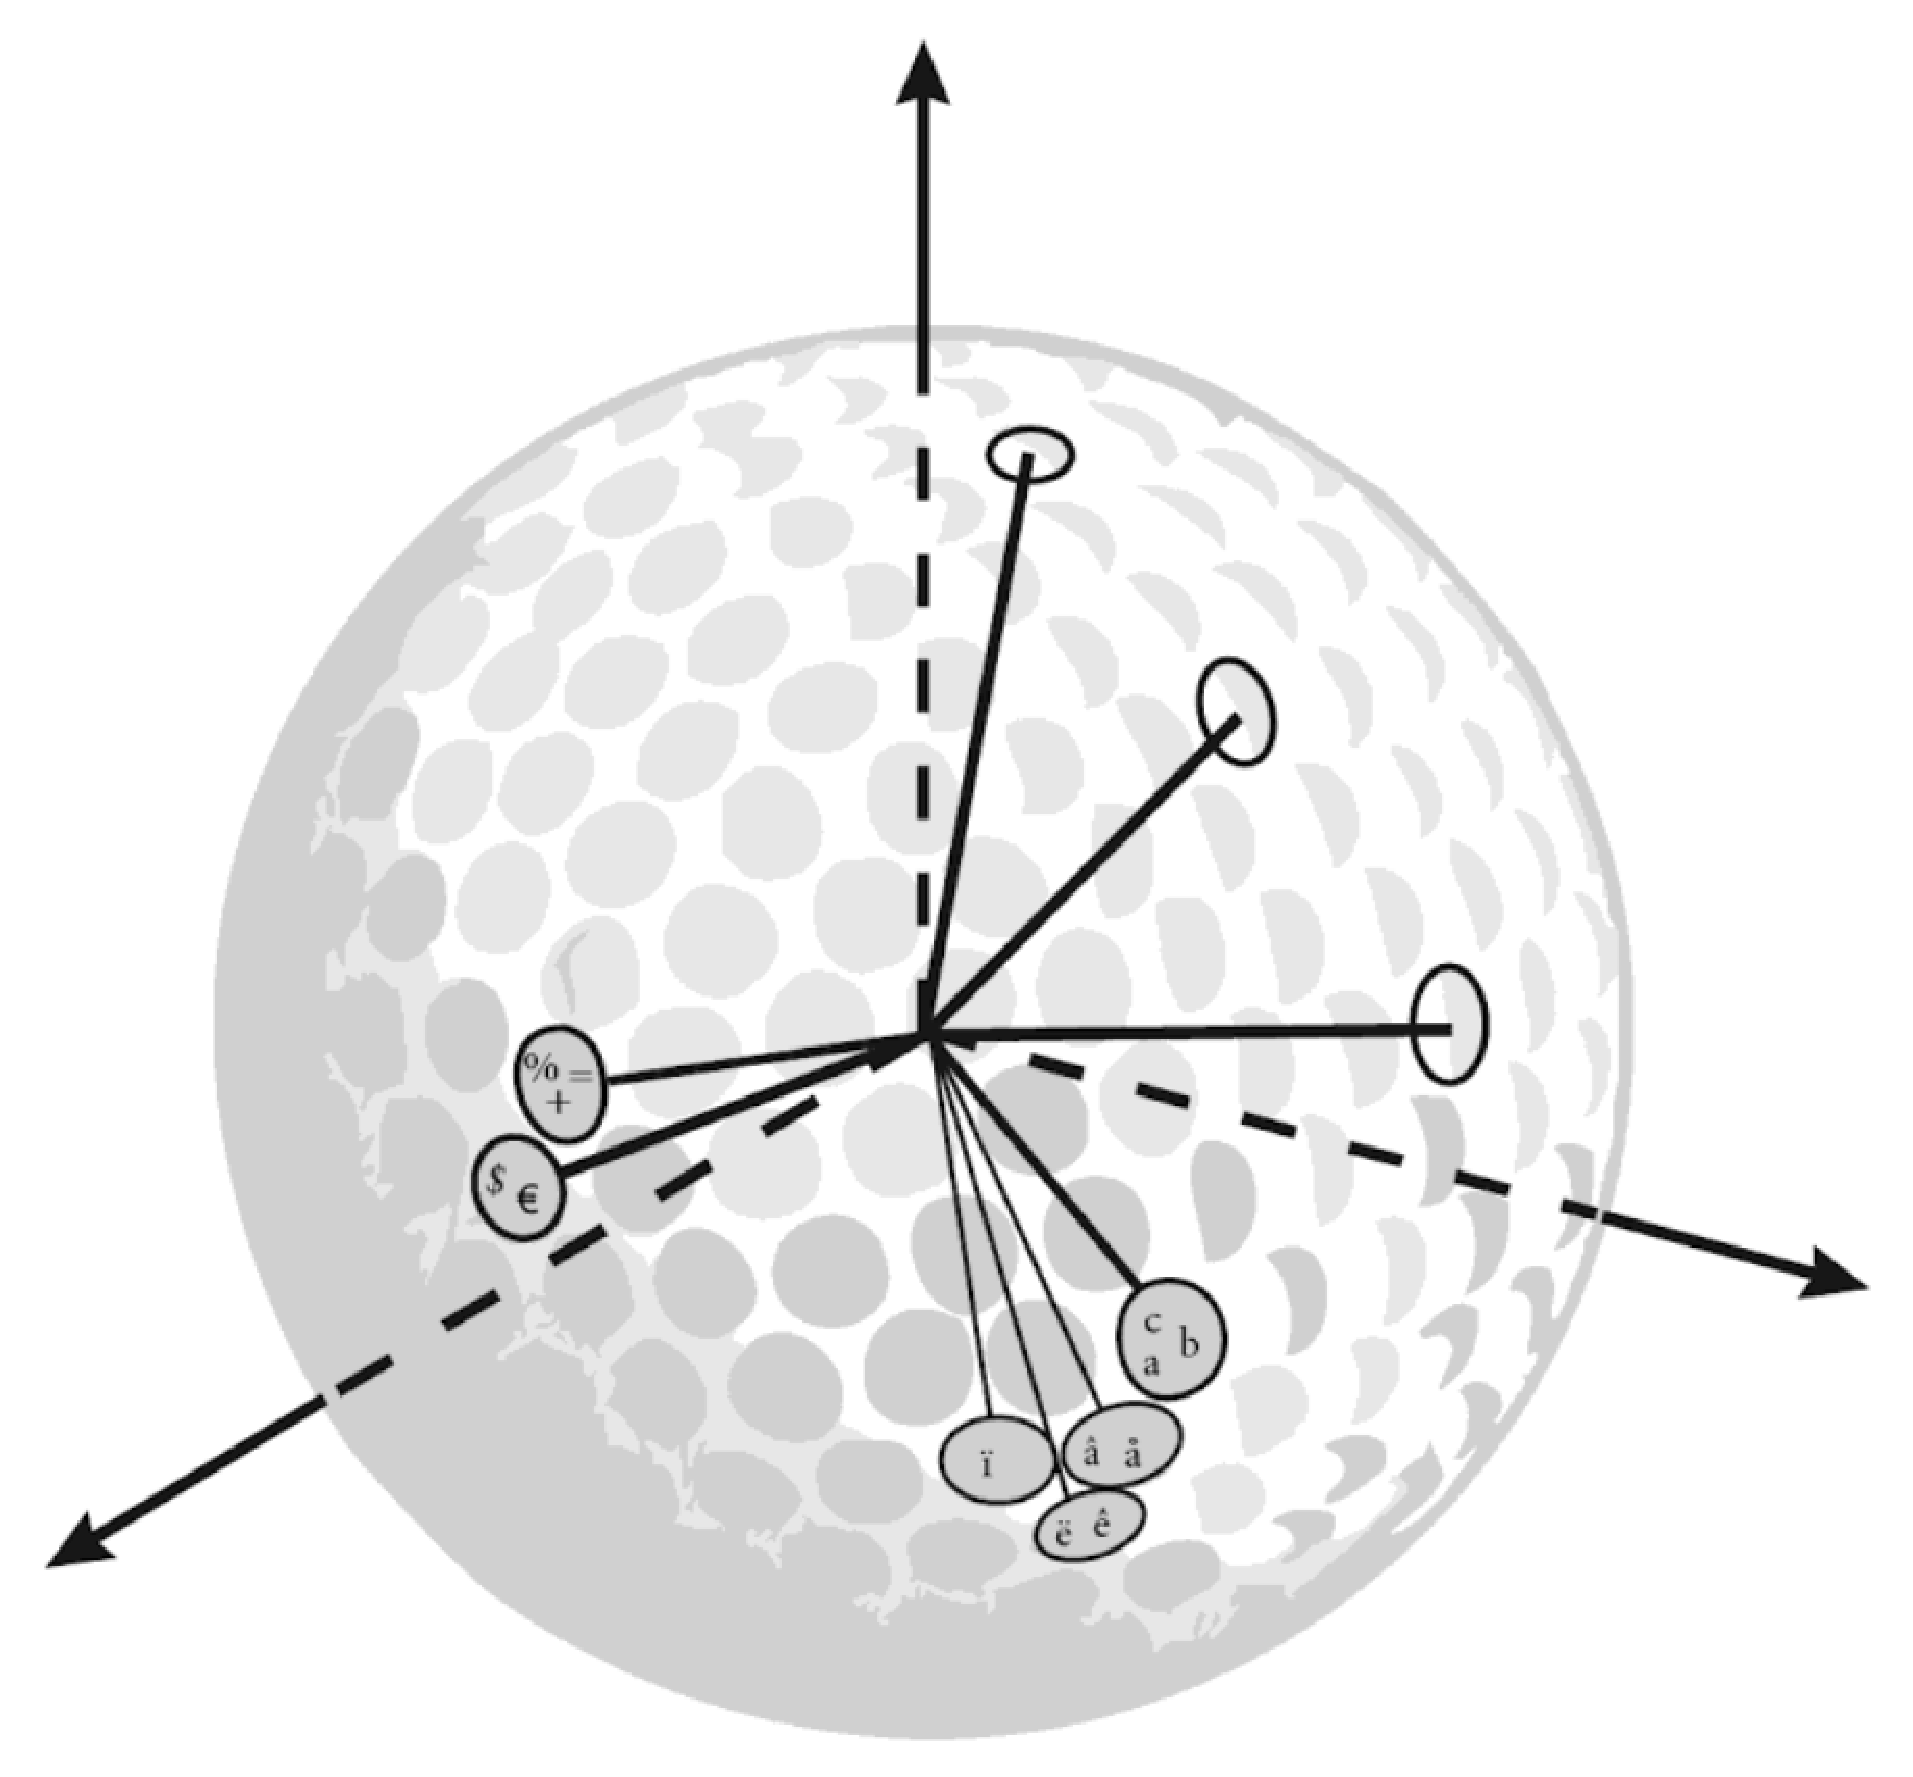
\includegraphics[width=0.45\textwidth]{imgs/conceptual_golfball.eps}
	}
	\subfloat[\label{subfig:constructed_vocab_sims}]{%
		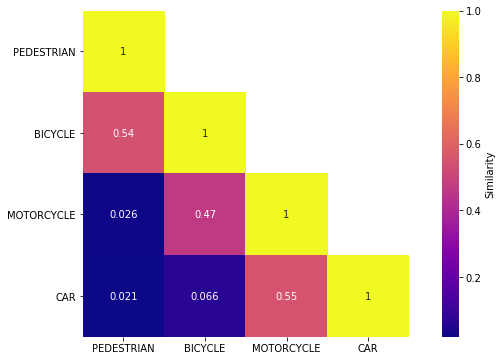
\includegraphics[width=0.45\textwidth]{imgs/SPA_constructed_vocab_sim.png}
	}
	\caption{Aspects of vector vocabularies:~\ref{subfig:conceptual_golfball} "Conceptual golf ball" depicting the idea of semantic vectors. Image source \cite{Eliasmith2013}.~\ref{subfig:constructed_vocab_sims} Cosine similarities in a small, manually engineered vector vocabulary of dimension $256$.}\label{fig:vector vocabs}
\end{figure}

Let $\vartheta \subset \mathcal{S}(D)$ be a vocabulary in the $D$-dimensional \ac{SPA}, where each vector $v \in \vartheta$ represents one item (i.e., a symbol, word or concept) in the representational space.
The content and size, i.e., the items of interest to be represented in such a vocabulary and their number as well as the way the representing vectors are established is highly task-dependent.
In its simplest form, all vectors in the vocabulary are chosen at random.
This approach is feasible due to the properties of high-dimensional vector spaces (cf. Theorem~\ref{theorem:VSA_cossim_distribution} in section~\ref{sec:math_prop_vsas}) that the probability of randomly chosen vectors being dissimilar grows with vector dimension.
Therefore,  we have low probability of unintentionally confusing two different concept vectors.
However, this approach does not capture any similarities between items being represented.
Ideally, the goal is that the similarity between vectors in the vocabulary $\vartheta$ somewhat reflects the similarity between represented items.
Figure~\ref{subfig:conceptual_golfball} depicts this idea: one subset of the space is assigned to vectors representing letters whereas another subset contains vectors representing special characters.
For a small number of items, the simplest way to create a vocabulary respecting some kind of similarity is to manually engineer the desired properties from randomly chosen vectors.
Let us assume we want to derive representative vectors for four different classes of traffic participants, namely \emph{pedestrian}, \emph{bicycle}, \emph{motorcycle},  and \emph{car}.
A simple structured vocabulary could be constructed in the following way
\begin{align*}
\mathbf{PEDESTRIAN} &:= \mathbf{DRIVE} \varoast \mathbf{MUSCLE} + \mathbf{ACTUATOR} \varoast \mathbf{LEG} \varoast \mathbf{TWO} \\
\mathbf{BICYCLE} &:= \mathbf{DRIVE} \varoast \mathbf{MUSCLE} + \mathbf{ACTUATOR} \varoast \mathbf{WHEEL} \varoast \mathbf{TWO}\\
\mathbf{MOTORCYCLE} &:= \mathbf{DRIVE} \varoast \mathbf{MOTOR} + \mathbf{ACTUATOR} \varoast \mathbf{WHEEL} \varoast \mathbf{TWO}\\
\mathbf{CAR} &:= \mathbf{DRIVE} \varoast \mathbf{MOTOR} + \mathbf{ACTUATOR} \varoast \mathbf{WHEEL} \varoast \mathbf{FOUR},
\end{align*}
with $\mathbf{DRIVE}$, $\mathbf{MUSCLE}$, $\mathbf{MOTOR}$, $\mathbf{ACTUATOR}$, $\mathbf{LEG}$, $\mathbf{WHEEL}$, $\mathbf{TWO}$ and $\mathbf{FOUR} \in \mathcal{S}(D)$ all being atomic vectors chosen at random.
Figure~\ref{subfig:constructed_vocab_sims} shows the similarities in an example vocabulary in $\mathcal{S}(256)$ constructed in the aforementioned way.
This vocabulary is designed to map simple motion properties into a vector representation.
Thus, this manually engineered vocabulary yields the desired property that vulnerable road users (in this case pedestrians and bicyclists) are more similar to each other that motor vehicles, whereas there is also similarity between different types of cyclists.
This approach allows the engineer to encapsulate almost any desired kind of similarity without loosing transparency during the encoding process, meaning that the reason for certain similarity artifacts is traceable.
However, not only does this approach become impracticable with increasing number of items in the vocabulary, it is also prone to biases imposed by the preferences of the human engineer.

A more sophisticated way to create a vector vocabulary is to learn it automatically from data.
In contrast to purely random vocabularies, the idea here is that the learning system is able to capture the intrinsic similarity between objects in the vector representation.
Again, the choice of learning paradigm (supervised vs.\ unsupervised) and architecture (e.g. \acp{CNN} or \acp{SOM}) depends not only on the given task, but also on the kind of similarity the vectors should encapsulate.
This can be visual similarity (e.g.\ items or objects that "look" similar), auditory similarity (e.g.\ objects producing similar sound), semantic similarity (e.g.\ words with similar meaning) or similarity in characteristics (e.g.\ similar motion characteristics).

A typical way of learning a vocabulary whose vectors conserve visual similarity in supervised fashion are \acp{CNN}.
These network architectures are inspired by the human visual cortex and compress high-dimensional visual input to lower dimensional representations.
They usually consist of a series of convolutional and pooling layers followed by one or more fully connected layers, where the last layer provides the classification result (cf.\ figure~\ref{subfig:cnn_arch}).
The activity of the second to last layer (the last fully-connected one before the actual classification) for each known class in the data set can be considered a representational vector for the current visual input.
A simple way of getting a representative vector for each class is simply calculating the element-wise, normalized mean over all examples in the test set.
We employ this approach in section~\ref{subsec:visual_vocabularies} to generate vocabularies encapsulating the visual similarity of traffic signs and traffic participants.
\begin{figure}[t]
	\centering
	\resizebox{.9\textwidth}{!}{%
	\begin{tikzpicture}[%
	auto,
	multilayer,
	]
	% \Plane[x=0, y=0, width=5, height=2, opacity=1, style={dashed, color=red}, NoFill]
	\node[line width=1mm] (input) at (0,-6)
	{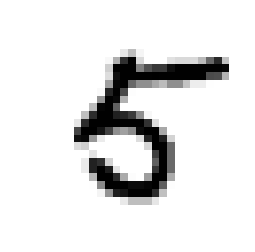
\includegraphics[width=.15\textwidth]{imgs/mnist.png}};
	\draw[thick] (0,-5) -- (0.75, -3);
	\draw[thick] (0,-5) -- (0.25, -2.8);
	\draw[thick] (0,-5) -- (-0.25, -2.6);
	\draw[thick] (0,-5) -- (-0.75, -2.4);
	% \begin{Layer}[layer=1]
	% 	\draw[very thick] (0,0) rectangle (5,2);
	% 	\node at (-.5,-.5)[below right]{Layer 1};
	% \end{Layer}
	\Vertices{data/cnn_vertices.csv};
	\Vertices[Pseudo]{data/last_cnn_vertices.csv};
	\Edges{data/cnn_edges.csv}
	\Edge[Direct](41)(45)
	\Edge[Direct](42)(46)
	\Edge[Direct](43)(47)
    \Edge[Direct](44)(48)
    \path (36.north) -- (37.south) 
      node[midway, sloped, draw=red, 
           ellipse, 
           rotate=60,
           fit=(35)(38), 
           inner sep=2pt,
           xslant=-0.5,
           yslant=-0.5,
           ]{};
	\end{tikzpicture}
	}
	\caption{A schematic visualization of a \ac{CNN} network architecture with the second to last layer, whose activity can be considered a compressed, lower-dimensional representation of the high-dimensional visual input, highlighted by a red ellipsis.}
	\label{fig:cnn_arch}
\end{figure}
A similar approach to derive vectors representing digits from $0$ to $9$ was used for the network performing the visual digit recognition task as part of the larger \ac{Spaun} model \cite{Eliasmith2012}, which was derived by training a \ac{DBN} consisting of four \acl{RBM} layers.
This approach of using the activity of the second to last layer to generate a atomic representational vectors can be generalized to any neural network for classification with dense layers at the end.

The aforementioned approach to create vector vocabularies encapsulating similarity by using neural networks, which are trained in supervised fashion, is suitable for capturing visual or auditory similarity structure in a vectors.
The generation of representational vectors for related or similar words or more generally semantic similarity in language is a problem often referred to as word embedding, which is a research question related to computational \acl{NLP}.
The most successful approaches such as \textit{word2vec} \cite{Mikolov2013a, Mikolov2013} or \textit{\ac{GloVe}} \cite{Pennington2014} typically use large corpora of text as input data and are trained in unsupervised fashion based on co-occurrence statistics of words.
The objective of those procedures aims at maximizing the dot product of word vectors that appear often in similar contexts while minimizing it for negative samples (which do not occur in the training data and are sampled at random).
For a given sentence $S=\left\{w_1, \ldots, w_n\right\}$ a context $C(w)$ of a word $w=w_i$ of size $k$ is a dynamic window of the form $C(w) = \left\{ w_{i-k}, \ldots, w_{i-1}, w_{i+1}, \ldots, w_{i+k}\right\}$.
The underlying assumption is that words sharing many contexts are similar to each other, such that automated training with the aforementioned objective will produce a good word embedding.
Surprisingly, these learning procedures lead to linguistic regularities and algebraic relations between word vectors \cite{Mikolov2013b}.
A common example is visualized in figure~\ref{fig:word2vec}: subtracting the vector representing $\mathbf{MAN}$ from the one representing $\mathbf{KING}$ and adding the vector representing $\mathbf{WOMAN}$ results in a vector most similar to the one representing $\mathbf{QUEEN}$, i.e., $\mathbf{KING} - \mathbf{MAN} + \mathbf{WOMAN} \approx \mathbf{QUEEN}$.
\begin{figure}[t]
	\centering
	\begin{tikzpicture}[%
	auto,
	scale=5,
	axis/.style={very thick, ->, >=stealth'},
	red line/.style={thick, ->, >=stealth', color=red},
	green line/.style={thick, ->, >=stealth', color=green},
	blue line/.style={thick, ->, >=stealth', color=blue},
	dashed blue line/.style={dashed, thick, color=blue},
	important line/.style={thick},
	dashed line/.style={dashed, thin},
	pile/.style={thick, ->, >=stealth', shorten <=2pt, shorten>=2pt},
	every node/.style={color=black}
	]
	% Draw axes
	% axis
	\draw[axis] (-0.5,0)  -- (1.2,0) node(xline){};
	\draw[axis] (0,-0.1) -- (0,1.1) node(yline){};
	\draw[red line] (0,0) -- (0.3, 0.8) node(King) [above right] {$\mathbf{KING}$};
	\draw[red line] (0,0) -- (0.7, 0.4) node(Man) [above right] {$\mathbf{MAN}$};
	\draw[green line] (0,0) -- (0.7, 0.9) node(Queen) [above right] {$\mathbf{QUEEN}$};
	\draw[green line] (0,0) -- (1.1, 0.5) node(Woman) [above right] {$\mathbf{WOMAN}$};
	\draw[blue line] (0,0) -- (-0.4, 0.4) node(KingMinusMan) [above] {$\mathbf{KING} - \mathbf{MAN}$};
	\draw[dashed blue line] (0.7,0.4) -- (0.3, 0.8);
	\draw[dashed blue line] (0.7,0.9) -- (1.1, 0.5);

	\end{tikzpicture}
	\caption{A typical example illustrating the semantic similarity structure between vectors representing the words \emph{king}, \emph{queen}, \emph{man} and \emph{woman} learned by Word2Vec allowing algebraic manipulation of the encoded entities. 
    Image inspired from \cite{Mikolov2013b}.}
	\label{fig:word2vec}
\end{figure}
However, the formal reasons for successful learning of word embeddings of those approaches are not well understood \cite{Goldberg2014, Levy2015}.

\subsection{Encoding structure}
\label{subsec:encoding_struct}

In section~\ref{subsec:vocabs}, we have already seen that there are many ways to create vector vocabularies that encode different types of similarity.
However, the strength of \acp{VSA} lies in the possibility to build up structured representations from atomic vectors.
Unordered sets can be represented by simply adding up atomic vectors.
Through the properties of the similarity measure, the sum is similar to each vector contained in the sum.
The most common approach to incorporate structure is to use so-called role-filler pairs \cite{Gayler2003}.
Such a pair is combined via the \ac{VSA}'s binding operation, where one vector of the pair takes the role of a variable while the other one can be considered the value of the variable.
We have already seen a simple example of this approach in section~\ref{subsec:vocabs}, where a small vocabulary representing four different classes of traffic participants was manually created.
In \ac{NLP} applications, this approach is useful when building up vectors representing phrases from a word vector vocabulary.
The phrase \textit{The dog chases the boy} could be encoded in a vector as
\begin{equation*}
	\mathbf{agent} \varoast \mathbf{dog} + \mathbf{verb} \varoast \mathbf{chase} + \mathbf{theme} \varoast \mathbf{boy},
\end{equation*}
assuming we already have a vocabulary containing atomic vectors representing those items.
Another typical example of this approach is the encoding of relations between items, such as "$\mathbf{A}$ is the mother of $\mathbf{B}$".
This relation could be represented in vectors through
\begin{equation*}
	m \left(\mathbf{A}, \mathbf{B} \right) = \mathbf{motherof} + \mathbf{mother} \varoast \mathbf{A} + \mathbf{child} \varoast \mathbf{B}.
\end{equation*}
The strength of \acp{VSA} is that the vectors representing such relations can subsequently be manipulated and combined using the \ac{VSA}'s algebraic operations.
In \cite{Kanerva2000}, Kanerva shows that this approach can be used to create a system, that is able to infer one relation, which is induced by another relation, through learning from example.
Their example features the aforementioned \textit{mother of} relation, which induces the \textit{parent of} relation
\begin{equation*}
	p \left(\mathbf{A}, \mathbf{B} \right) = \mathbf{parentof} + \mathbf{parent} \varoast \mathbf{A} + \mathbf{offspring} \varoast \mathbf{B},
\end{equation*}
i.e., we have $m\left(\mathbf{A}, \mathbf{B}\right) \Longrightarrow p\left(\mathbf{A}, \mathbf{B}\right)$.
Combining several examples
\begin{equation*}
	M = \sum_{i=0}^{n} m\left(\mathbf{A}_i, \mathbf{B}_i \right) \varoast p\left(\mathbf{A}_i, \mathbf{B}_i \right)
\end{equation*}
yields a transition vector, which gives $ M \varoast m \left(\mathbf{X}, \mathbf{Y} \right) \approx p \left(\mathbf{X}, \mathbf{Y} \right)$ for unseen examples $\mathbf{X}$ and $\mathbf{Y}$.
However, this approach is based on the self-cancellation property (i.e., $\mathbf{X} \varoast \mathbf{X} = \pmb{1}$) in certain \acp{VSA} (in particular  \acp{BSC}), as it leads to $M$ containing the vector $\mathbf{motherof} \varoast \mathbf{parentof} + \mathbf{mother} \varoast \mathbf{parent} + \mathbf{child} \varoast \mathbf{offspring}$ (see \cite{Kanerva2000} for details).
A similar approach was used in \cite{Kleyko2015a} for a prototype of concept learning.
The authors in \cite{Rasmussen2011} employ a similar approach to encode a rule for inductive learning in a transition vector using the \ac{VSA}'s algebraic operations to solve \acp{RPM}.
The authors represent consecutive cells in an \ac{RPM} and encode the transition from one cell to another in a particular transition vector and, from a sequence of those, iteratively create a general transition vector encapsulating the general rule for going to the next cell in the matrix.
They implement these vectors as well as their inductive learning system in a \ac{SNN} model, a process we will also briefly discuss in the next section,

\subsection{Implementation in \aclp{SNN}}%
\label{subsec:implementation_in_snns}

In this section, we show how \acp{VSA} and in particular the \ac{SPA} can be implemented in \acp{SNN}.
In section~\ref{subsec:nef_representation}, we have already discussed the representation principle of the \ac{NEF}, that allows to encode time-varying vectors in the activity of populations of spiking neurons using equation~\eqref{eq:nef_encoding}.
Given that all representations of entities in the \ac{SPA} are vectors, we can directly apply equation~\eqref{eq:nef_encoding} to encode any vector representation generated using the principles and algebraic operations of the \ac{SPA}.
Similarly, we can employ equation~\eqref{eq:nef_decoding} to decode back out the original vector from the neurons' activities.
However, to manipulate the encoded vectors into structured representations using the \ac{SPA}'s algebraic operations, we also need to be able to implement these operations in networks of spiking neurons.
Again, the tools of the \ac{SPA} allow this implementation.
The implementation of element-wise addition of vectors is straightforward: assuming we have created a neural populations $A$ and $B$ encoding the vectors $ \mathbf{v}$ and $ \mathbf{w}$ respectively using equation~\eqref{eq:nef_encoding}, we can now use the transformation principle and equation~\eqref{eq:nef_transformation} to connect \emph{both} populations $A$ and $B$ to a third population $C$ with both connections approximating the identity function.
The population $C$ receiving input from both populations $A$ and $B$ will end up representing an approximation of the sum $ \mathbf{v}+ \mathbf{w}$.

Similarly, we can use the \ac{NEF}'s principles to implement the \ac{SPA}'s binding operation, circular convolution, in a network of spiking neurons.
Revisiting equation~\eqref{eq:conv_with_dft}, we can write the circular convolution of two vectors $ \mathbf{z} = \mathbf{v}, \mathbf{w}$ as

\begin{equation}
    \mathbf{z} = \mathbf{v} \varoast \mathbf{w} = \ac{IDFT}\left(\ac{DFT}( \mathbf{v}) \odot \ac{DFT}( \mathbf{w}) \right). \tag{\ref{eq:conv_with_dft} revisited}
\end{equation}

We can consider the \ac{DFT} and \ac{IDFT} as linear functions given by the matrices

\begin{equation}
\label{eq:dft_mat}
W = \frac{1}{ \sqrt{D-1}} \left(\zeta_{D} ^{i\cdot j}\right)_{i,j=0}^{D-1} \qquad
W^{-1} = \frac{1}{ \sqrt{D-1}} \left(\zeta_{D} ^{-i\cdot j}\right)_{i,j=0}^{D-1}
\end{equation}
and thus write circular convolution as matrix multiplication

\begin{equation}
\label{eq:circ_conv_mat}
\mathbf{z} = \mathbf{v} \varoast \mathbf{w} = W^{-1} \left( \left(W \mathbf{v}\right) \cdot \left(W \mathbf{w}\right)\right).
\end{equation}
Applying the \ac{NEF}'s transformation principle, we can implement circular convolution in a spiking neuron substrate.
To finally be able to unbind vectors, i.e., calculate $ \mathbf{v} = \mathbf{z} \varoast \bar{\mathbf{w}}$ using the pseudo-inverse element $ \bar{ \mathbf{w}} = \left(w_0, w_{D-1}, w_{D-2}, \ldots, w_{1}\right)$ (cf.\ Lemma~\ref{lemma:spa_pseudo_inv}), we can adapt equation~\eqref{eq:circ_conv_mat}.
The function transforming a vector into its pseudo-inverse element is a simple permutation of elements given by the matrix 
\begin{equation}
\label{eq:mat}
C_{pinv} = \left(
    \begin{matrix}
        1 & 0 &  \cdots & 0  & 0 \\
        0 & 0 &  \cdots & 0  & 1 \\
        0 & 0 &  \cdots & 1  & 0 \\
        \vdots & \vdots  & \iddots & \vdots  & \vdots \\
        0 & 1 &  0 & \cdots  & 0 
    \end{matrix}
\right),
\end{equation}
which allows us to transform equation ~\eqref{eq:circ_conv_mat} into
\begin{equation}
\label{eq:unbind_mat}
\mathbf{v} \approx \mathbf{z} \varoast \bar{ \mathbf{w}} = W^{-1} \left( \left(W \mathbf{z}\right) \cdot \left(W \cdot C_{pinv} \mathbf{w}\right)\right).
\end{equation}
The implementation of a \ac{SNN} performing a biologically plausible version of a cleanup memory employing the \ac{NEF} is shown in \cite{Stewart2011}.
Thus, applying the principles of the \ac{NEF}, we can represent the representational vectors of the \ac{SPA} in the activity of populations of spiking neurons and implement its algebraic operations in networks of spiking neuron populations.
A subtle detail worth noting with regard to implementing \acp{VSA} in \acp{SNN} is that the vectors used for representing concepts or entities of interest are \emph{not} vectors of neural activity.
That is, there are two distinct representational vector spaces: the space of neural activities (i.e., measurable properties like spike patterns) and the vector space used to generate the vocabulary and structured representations vectors which in turn are represented by the activities of populations in the neural space (see \cite{Eliasmith2013} for further details).

There are several reasons for implementing cognitive architectures like the \ac{SPA} in a spiking neuron substrate.
Regarding the application of vector-based representations in cognitive modeling, it makes sense to consider an implementation in neural activity, since the biological systems able to perform cognitive tasks are also systems of neural networks.
Hence, when generating models of some cognitive function or behavior such as the model for inductive rule generation applied to \acp{RPM} in \cite{Rasmussen2011}, implementation in a spiking neuron substrate allows to compare the model's neural activity with neural activity measured in the brain of human subjects performing a similar task.
Such a comparison enables more detailed model analysis and improvements by allowing researchers to draw inspirations from actual biological systems.
Considering applications of the \ac{SPA} in domains such as automated driving as proposed in later chapters~\ref{chap:driving_context_classification},~\ref{chap:behav_pred} and~\ref{chap:mix_online_learning}, the possibility of implementation in a spiking neuron substrate is particularly interesting in terms of energy-efficiency.
As discussed in section~\ref{sec:neuromorphic_HW}, there exists a growing number of neuromorphic hardware devices dedicated to efficiently processing networks of spiking neurons.
Such dedicated computing hardware allows to run \acp{SNN} more efficiently than traditional computing hardware, which often requires several orders of magnitude less energy \cite{Hunsberger2016}.
This is particularly interesting in mobile applications such as robotic systems or, more particularly, automated driving which poses increasingly strong restrictions on the energy-budget of individual components due to growing setups of both, on-board sensors and computing hardware.
Since these novel computing devices are not yet available as commercial products but rather prototypes developed in academic research, the deployment of the models developed in this thesis on neuromorphic computing hardware integrated into a vehicle's architecture is unfortunately out of scope of this thesis. 

\section{Summary}
In this chapter, we have introduced the theoretical background and mathematical properties of \aclp{VSA}, which is the basis for subsequent chapters.
Furthermore, we established a formal, mathematical notion for \acp{VSA} in general (section ~\ref{sec:math_prop_vsas}), which, to the best or our knowledge, is not available in the literature except for treatments of particular instantiations of \acp{VSA} such as in \cite{Plate1994}, \cite{Gayler1998} or \cite{Kanerva2009}.
The we shifted our focus to one particular \ac{VSA}, the \ac{SPA}, presenting its most important aspects and properties with respect to subsequent chapters of the thesis.
Furthermore, we gave a brief description of the \acl{NEF}, which is typically used to implement large-scale neural models of spiking neurons such as the one presented in \cite{Eliasmith2012}.
Finally, we have introduced the basic principles of cognitive modeling using \acp{VSA} in general and the \ac{SPA} in particular.
We showed several general approaches to generate vocabularies of atomic vectors, which form the basis of more complex structured representations built from them using the \ac{VSA}'s algebraic operations.
Finally, we connected the mathematical description and theory of both, the \acp{VSA} and the \ac{NEF} by depicting how the \ac{NEF} can be used to implement the \ac{SPA} in a spiking neuron substrate, which offers interesting possibilities regarding energy-efficiency in mobile applications such as automated driving.
We will use the theory and findings shown here in subsequent chapters to derive vector-based representations of automotive data measured and collected in actual driving situations to tackle tasks like classifying the current driving context or prediction the future development of the scene based on past observations.
